\section{Results}%
\label{sec:results}

The main outcome variables in my analysis are ``discretionary spend'', defined
as spend transactions over which users likely have a lot of control, and
``net-inflows into savings-accounts'', defined as the difference between
inflows into and outflows from all of a user's savings
accounts.\footnote{Discretionary spend is calculated solely based on card
    transactions, while cash transactions are excluded. This is because cash
    transactions are recorded in the MDB data as ATM withdrawals, and it is
    impossible to know what these funds were used for. Furthermore, I do
    not include gasoline expenses in discretionary spend because many people
    use their car to commute to work so that it is unclear what proportion of
    these expenses are discretionary. A list of transaction tags used to
    identify discretionary spend transactions and the code used create the
    variable are available on
    \href{https://github.com/fabiangunzinger/mdb_eval/blob/f31bfcd7a330188cdd27968d41957ebf5b454099/src/data/aggregators.py\#L389}{Github}.
    To capture only user-generated savings-account flows and not interest
    payments and similar automated transactions, I include only transaction
with an absolute value of \pounds5 or higher. The code used to calculate
savings account flows is also available on
\href{https://github.com/fabiangunzinger/mdb_eval/blobf31bfcd7a330188cdd27968d41957ebf5b454099/src/data/aggregators.py\#L89}{Github}.}


\subsection{Main results}%
\label{sub:main_results}

\begin{figure}[h]
    \centering 
    \caption{Main results}
    \label{fig:main_results}
    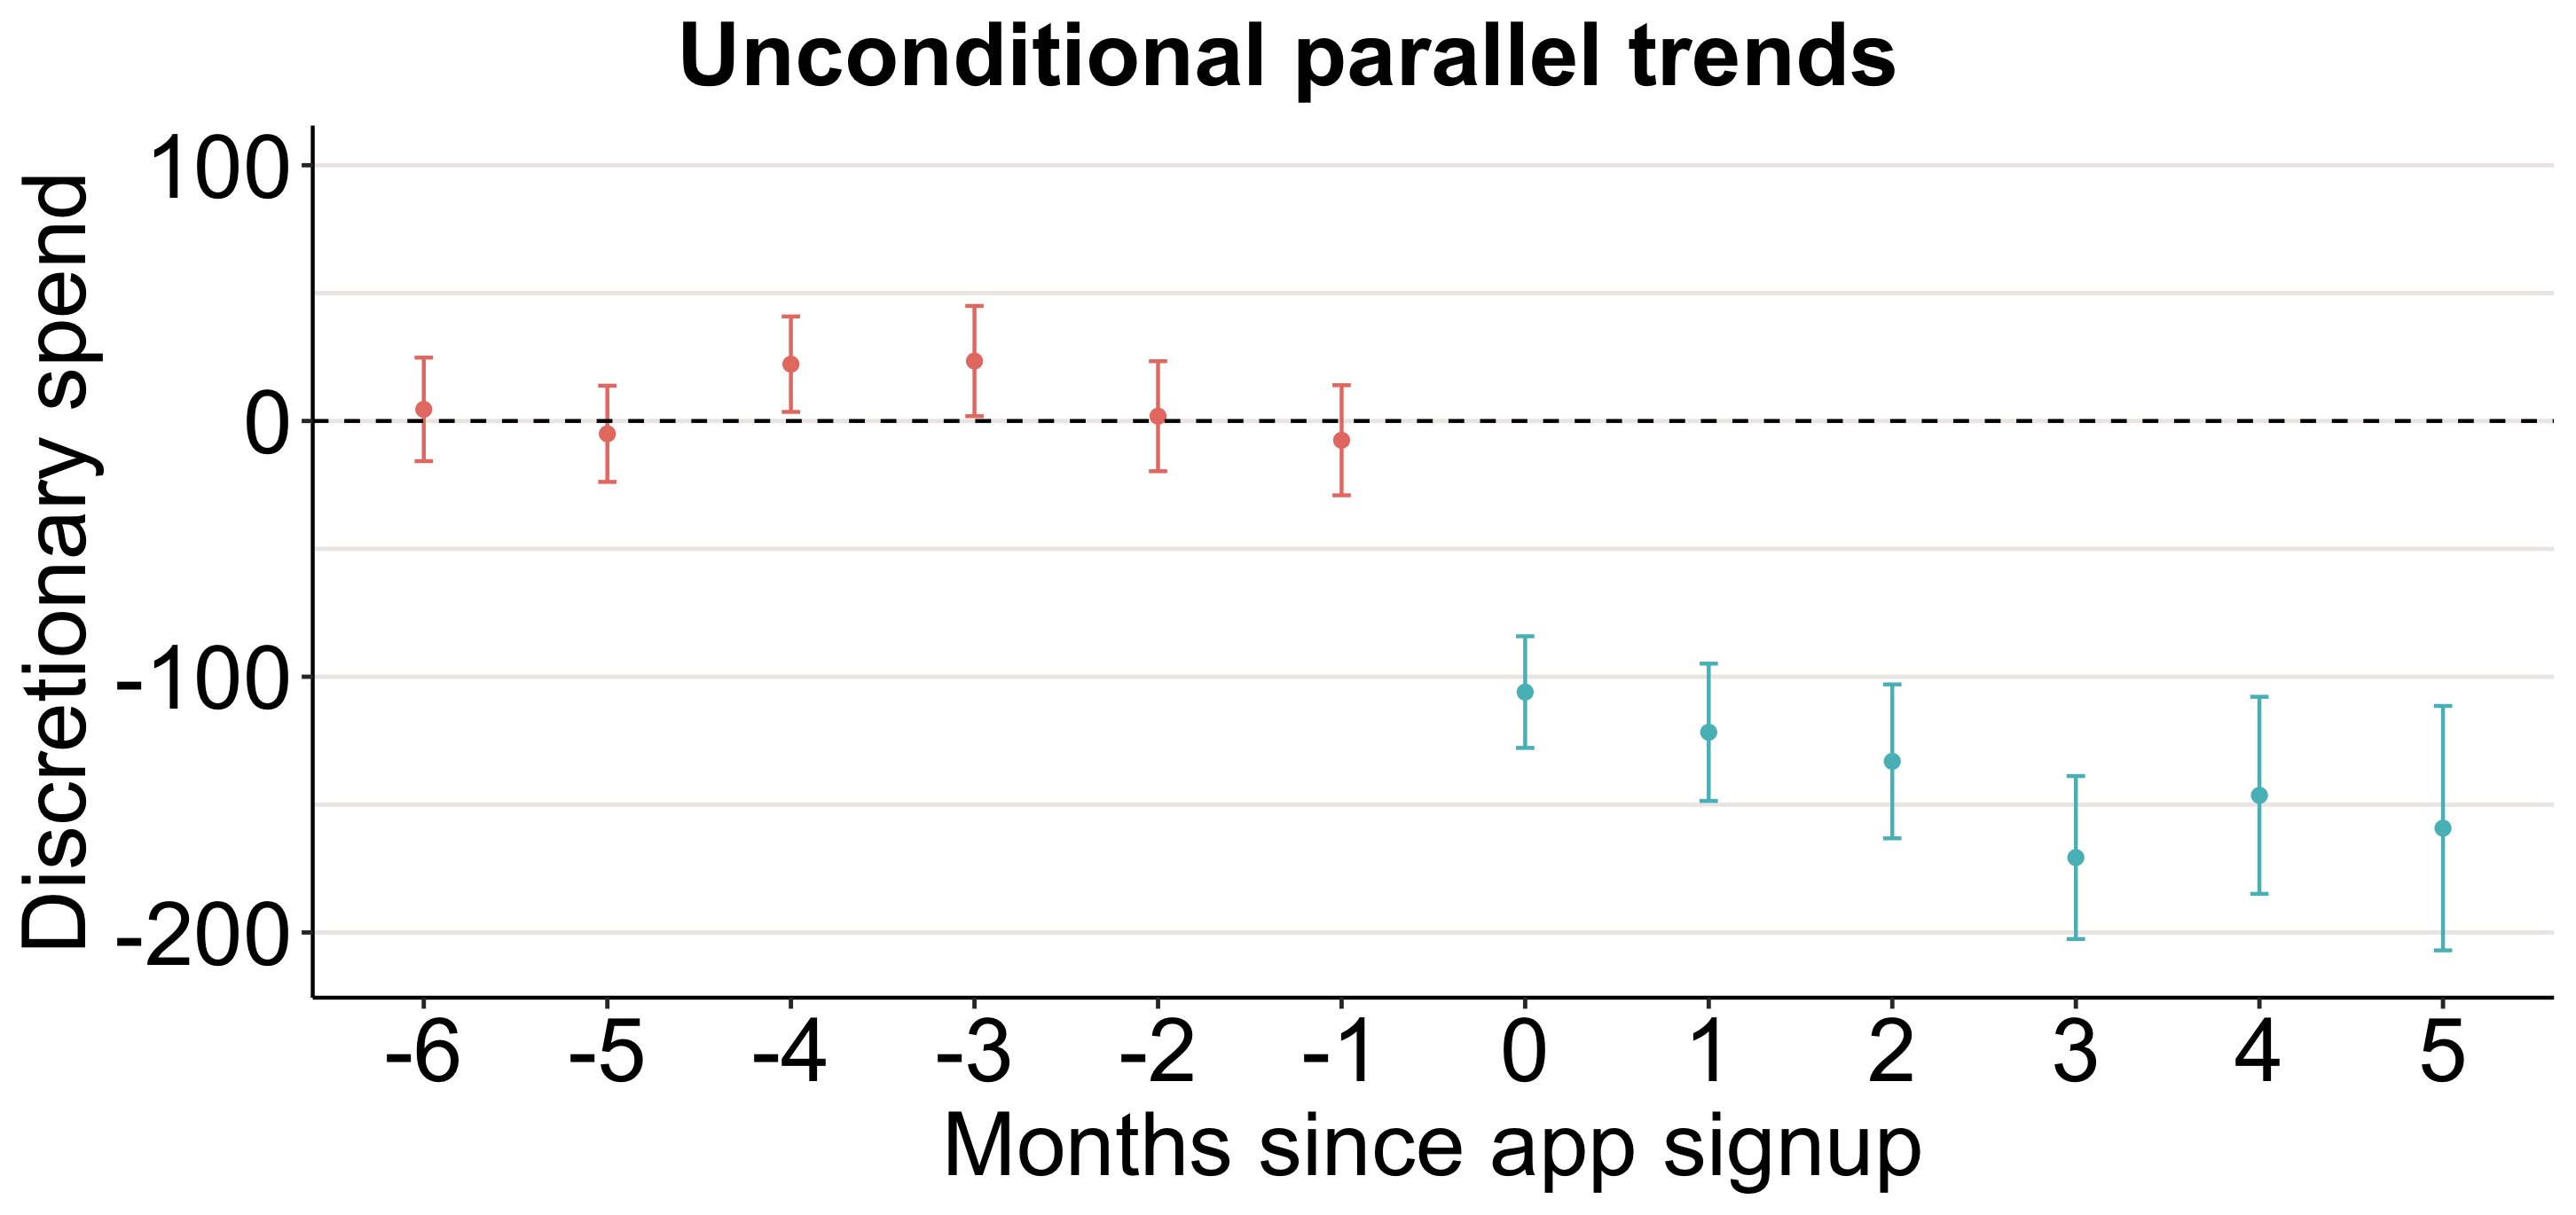
\includegraphics[width=.49\textwidth]{\figdir/dspend_uncond_es.png}
    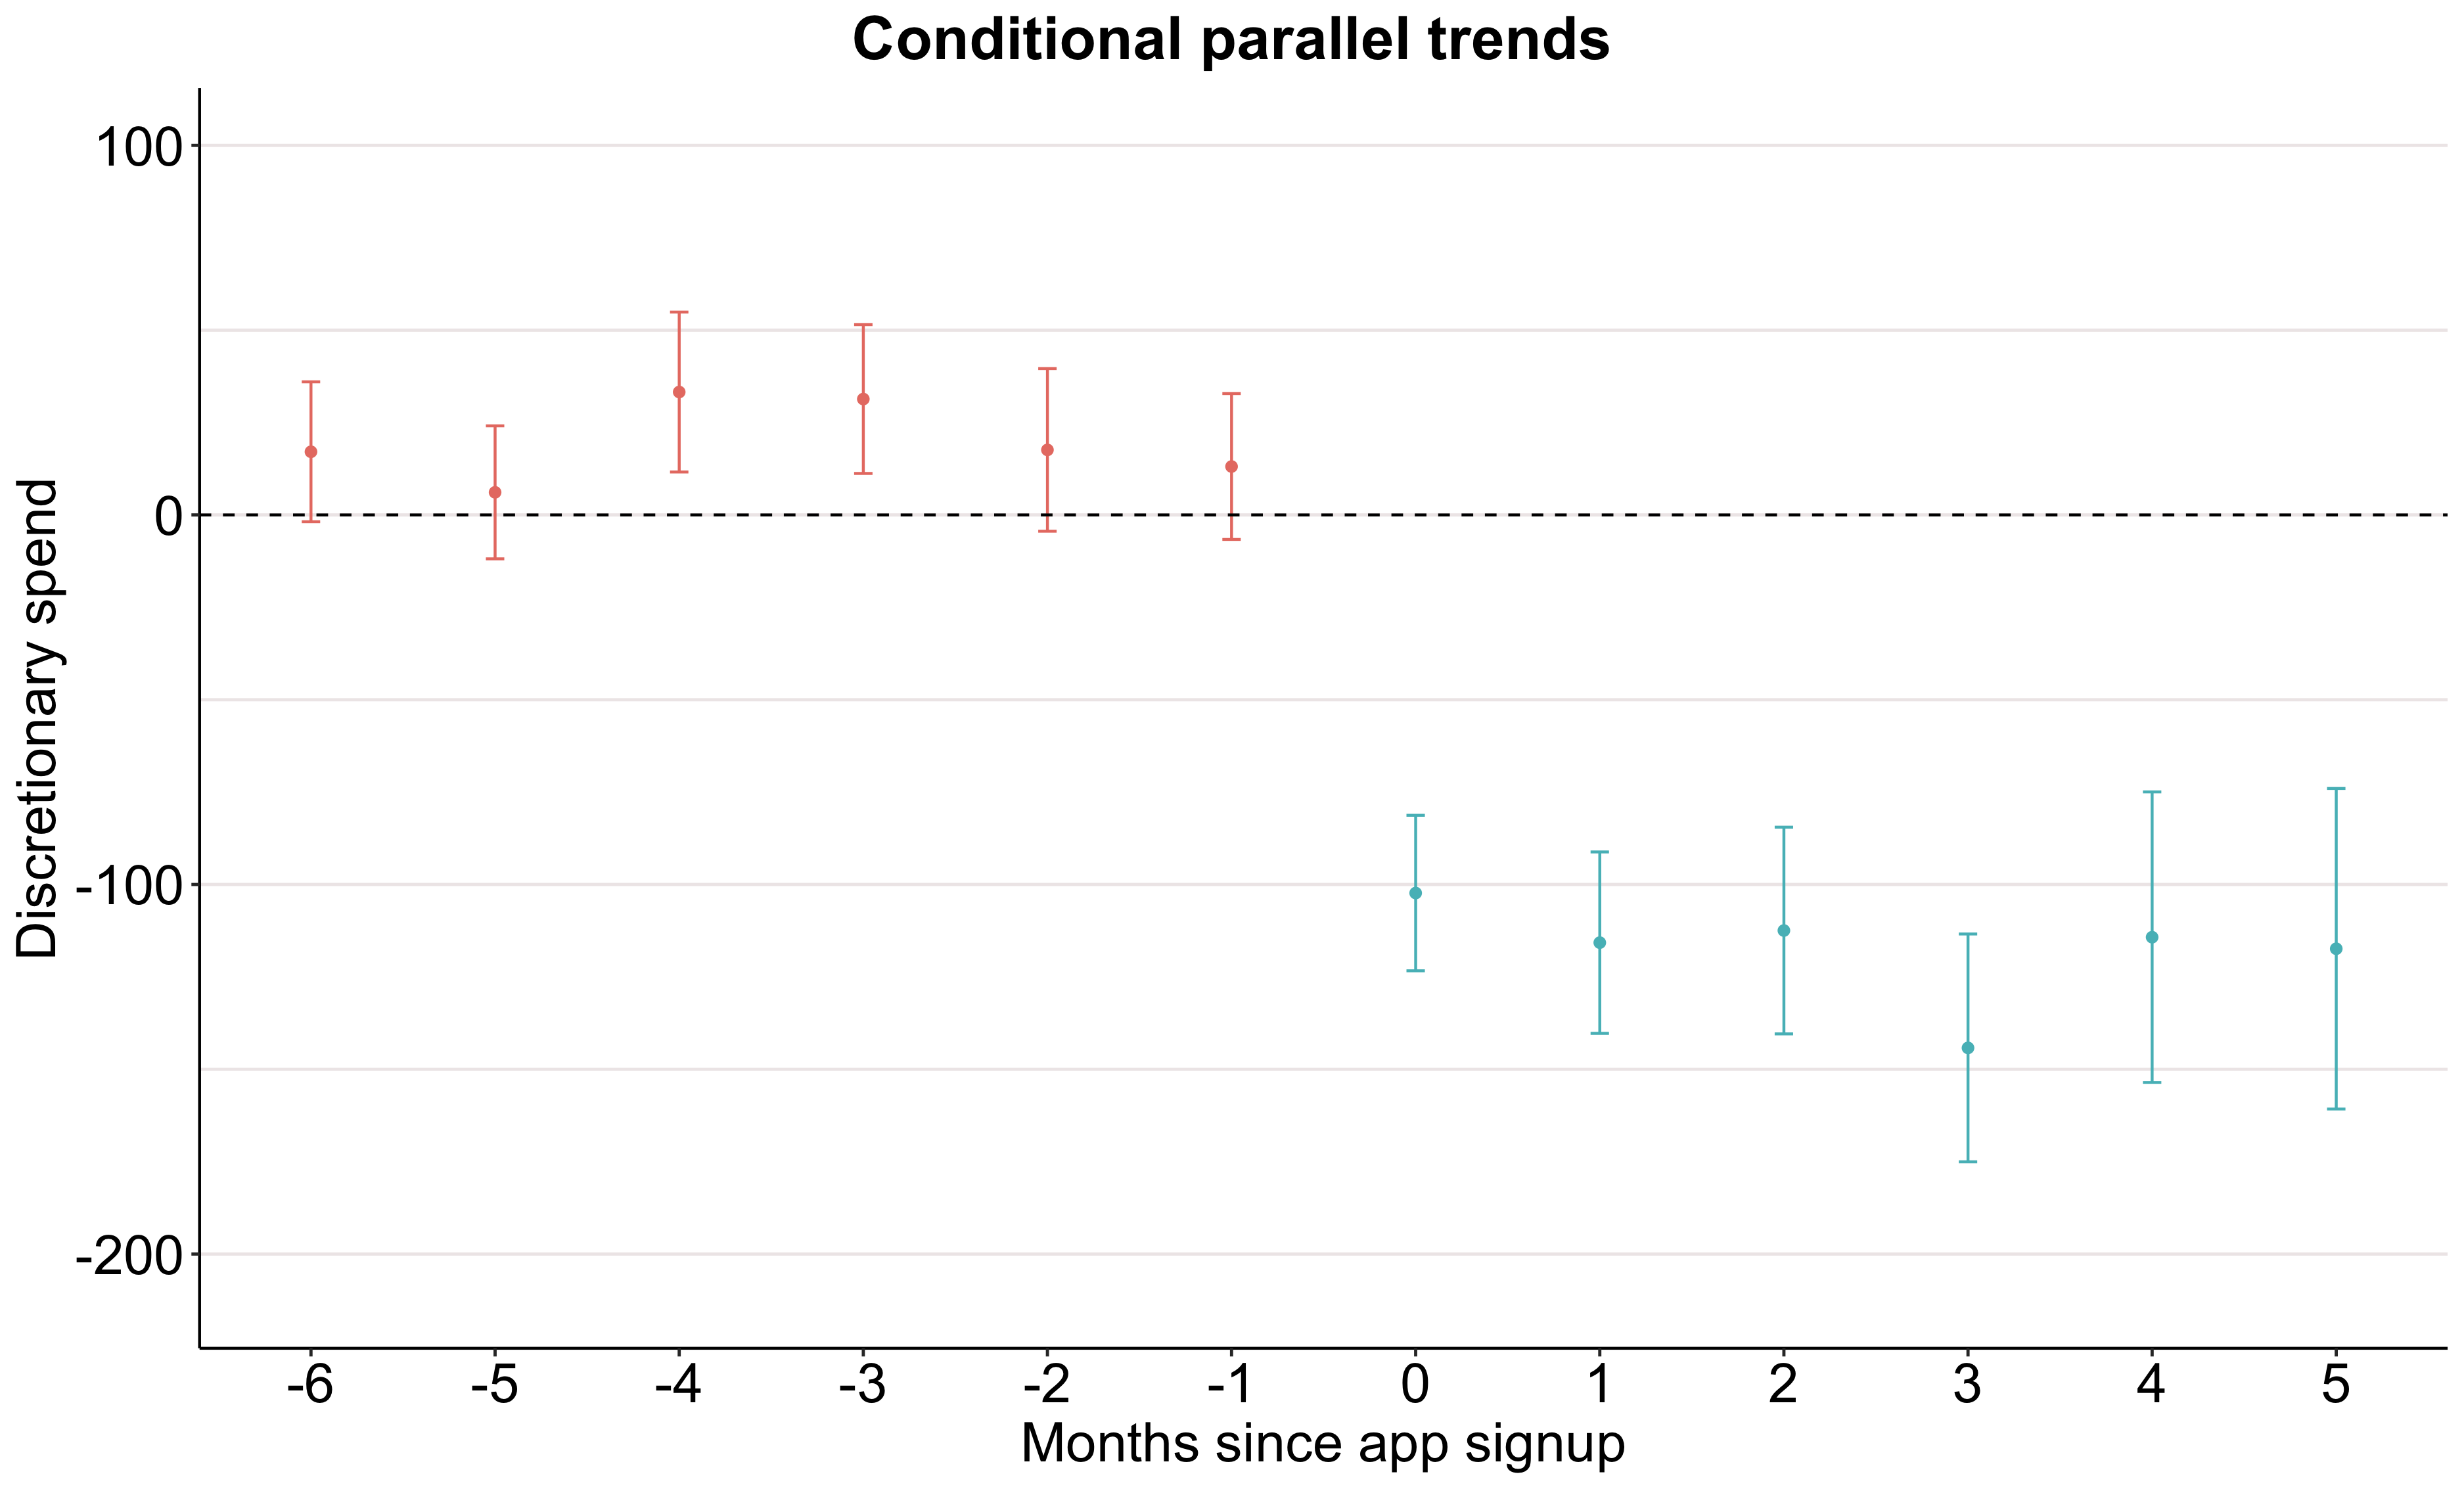
\includegraphics[width=.49\textwidth]{\figdir/dspend_cond_es.png}
    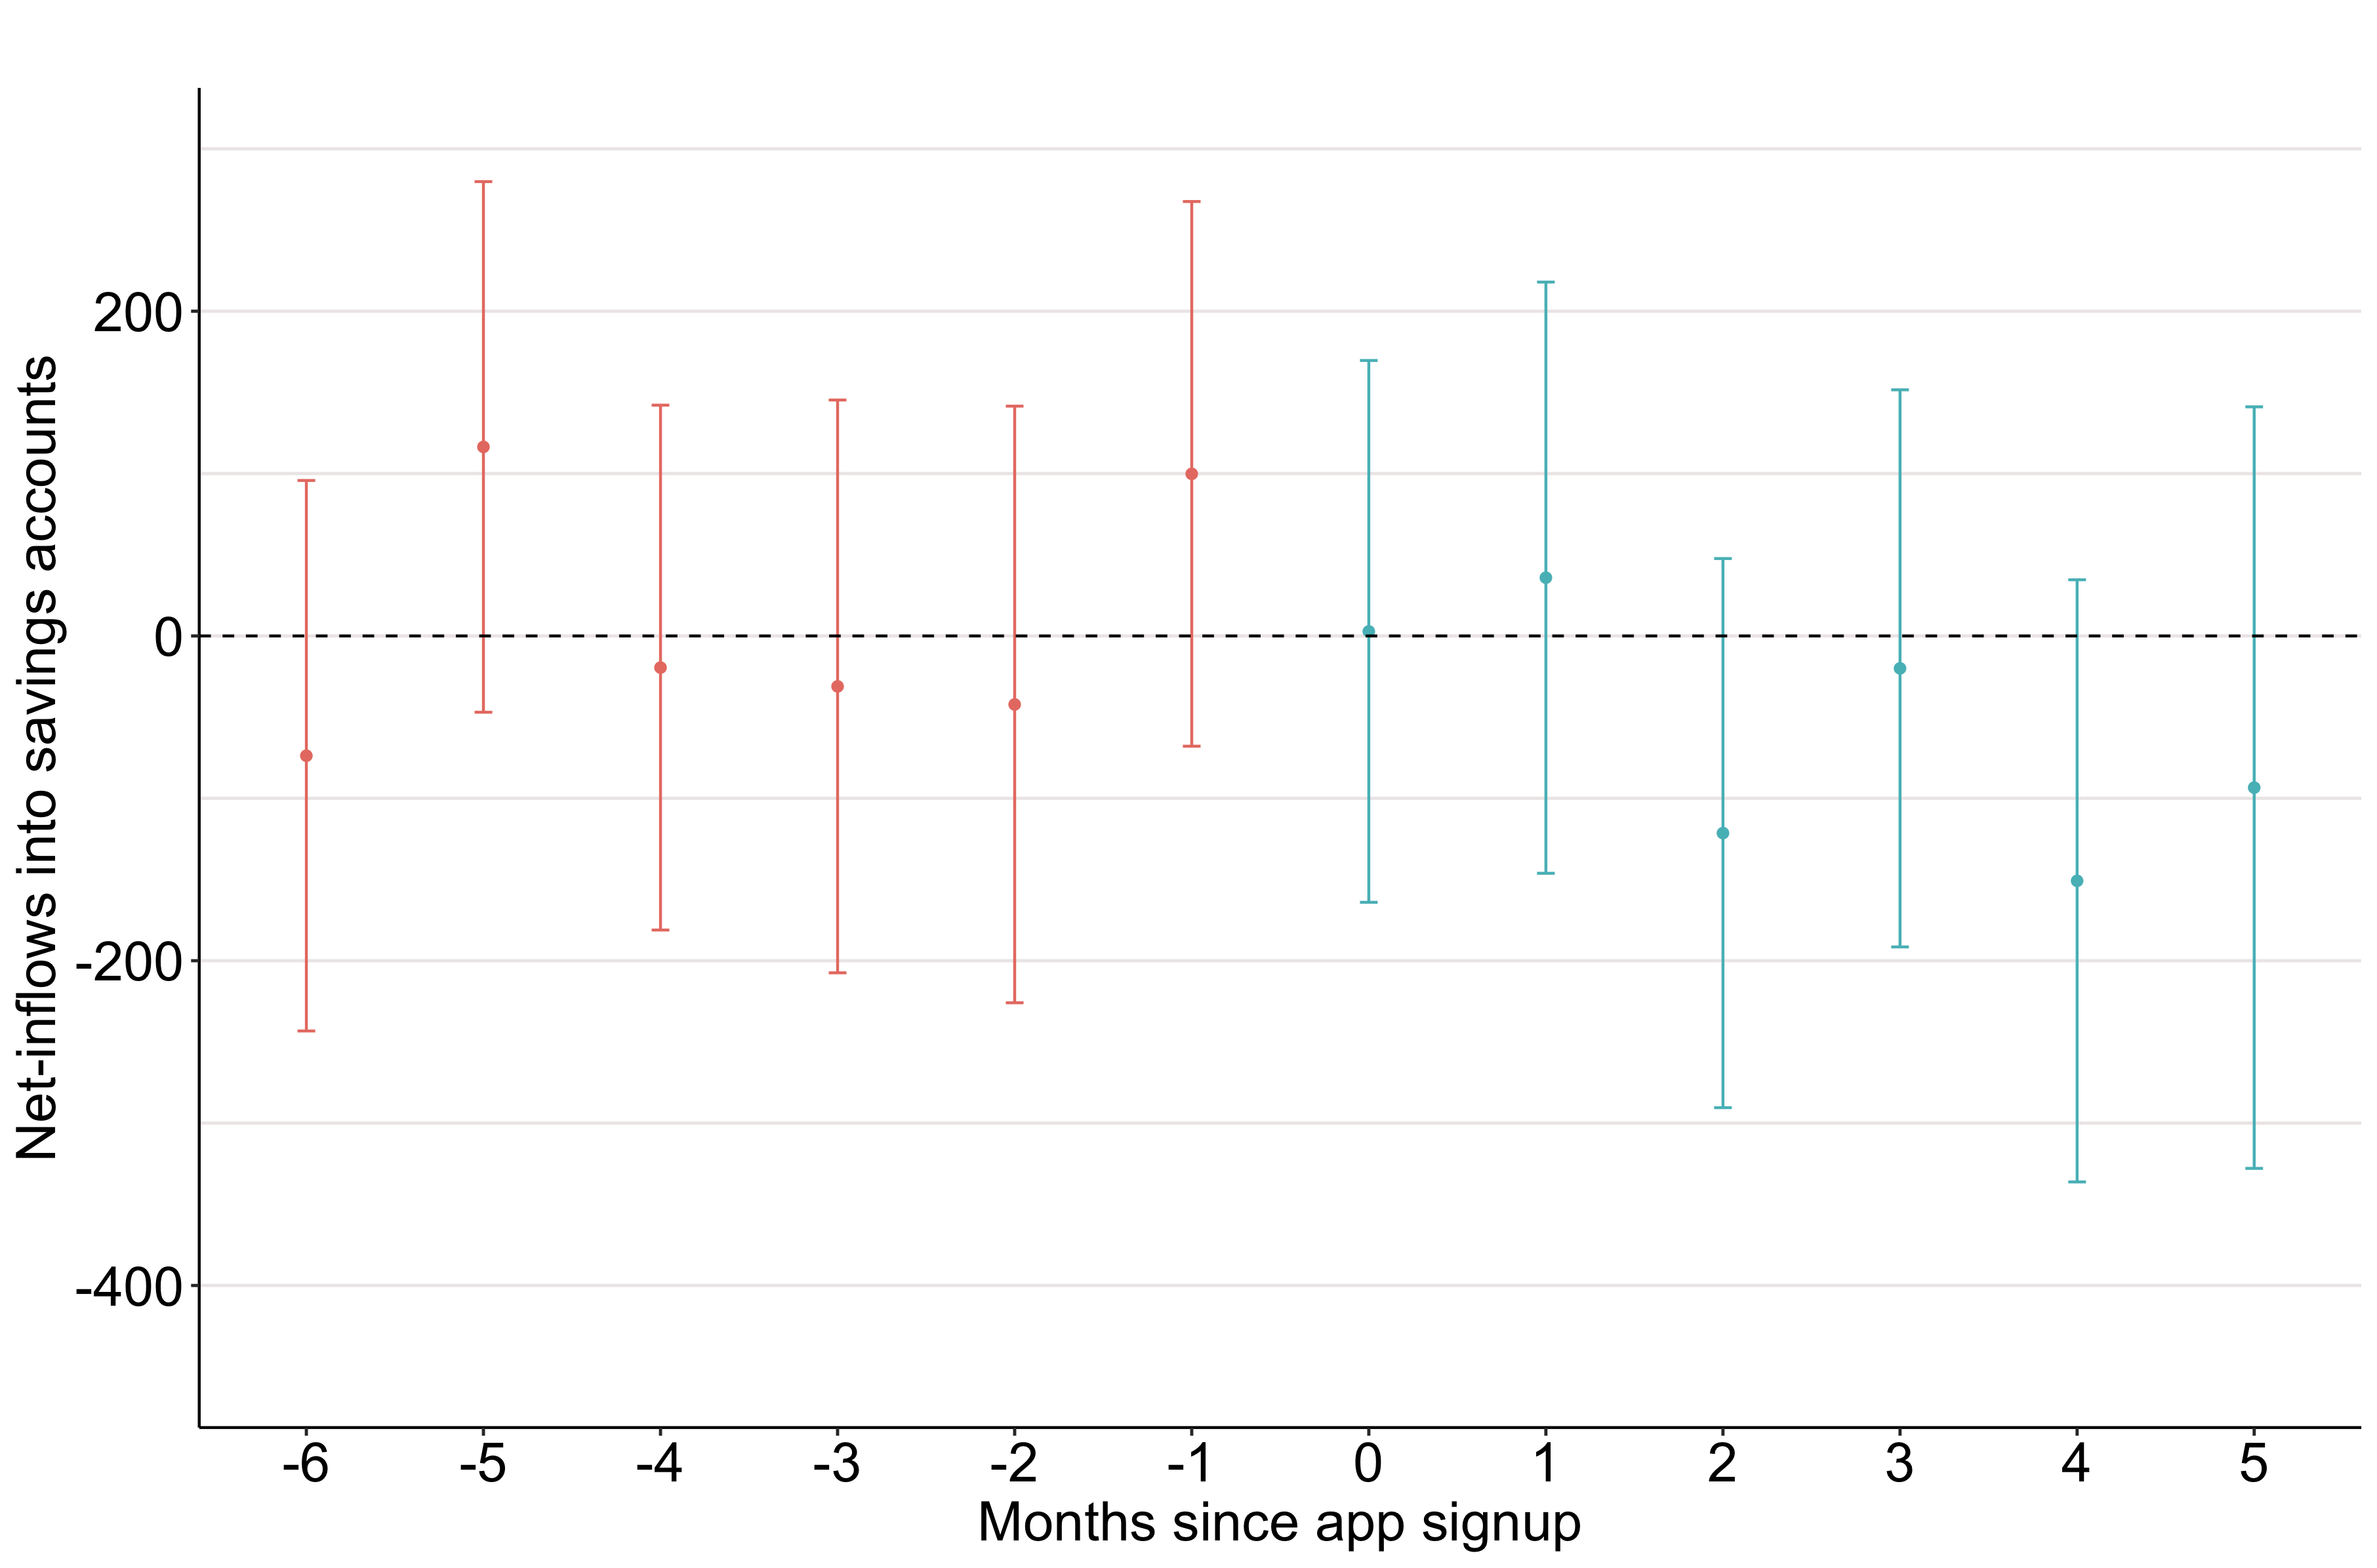
\includegraphics[width=.49\textwidth]{\figdir/netflows_uncond_es.png}
    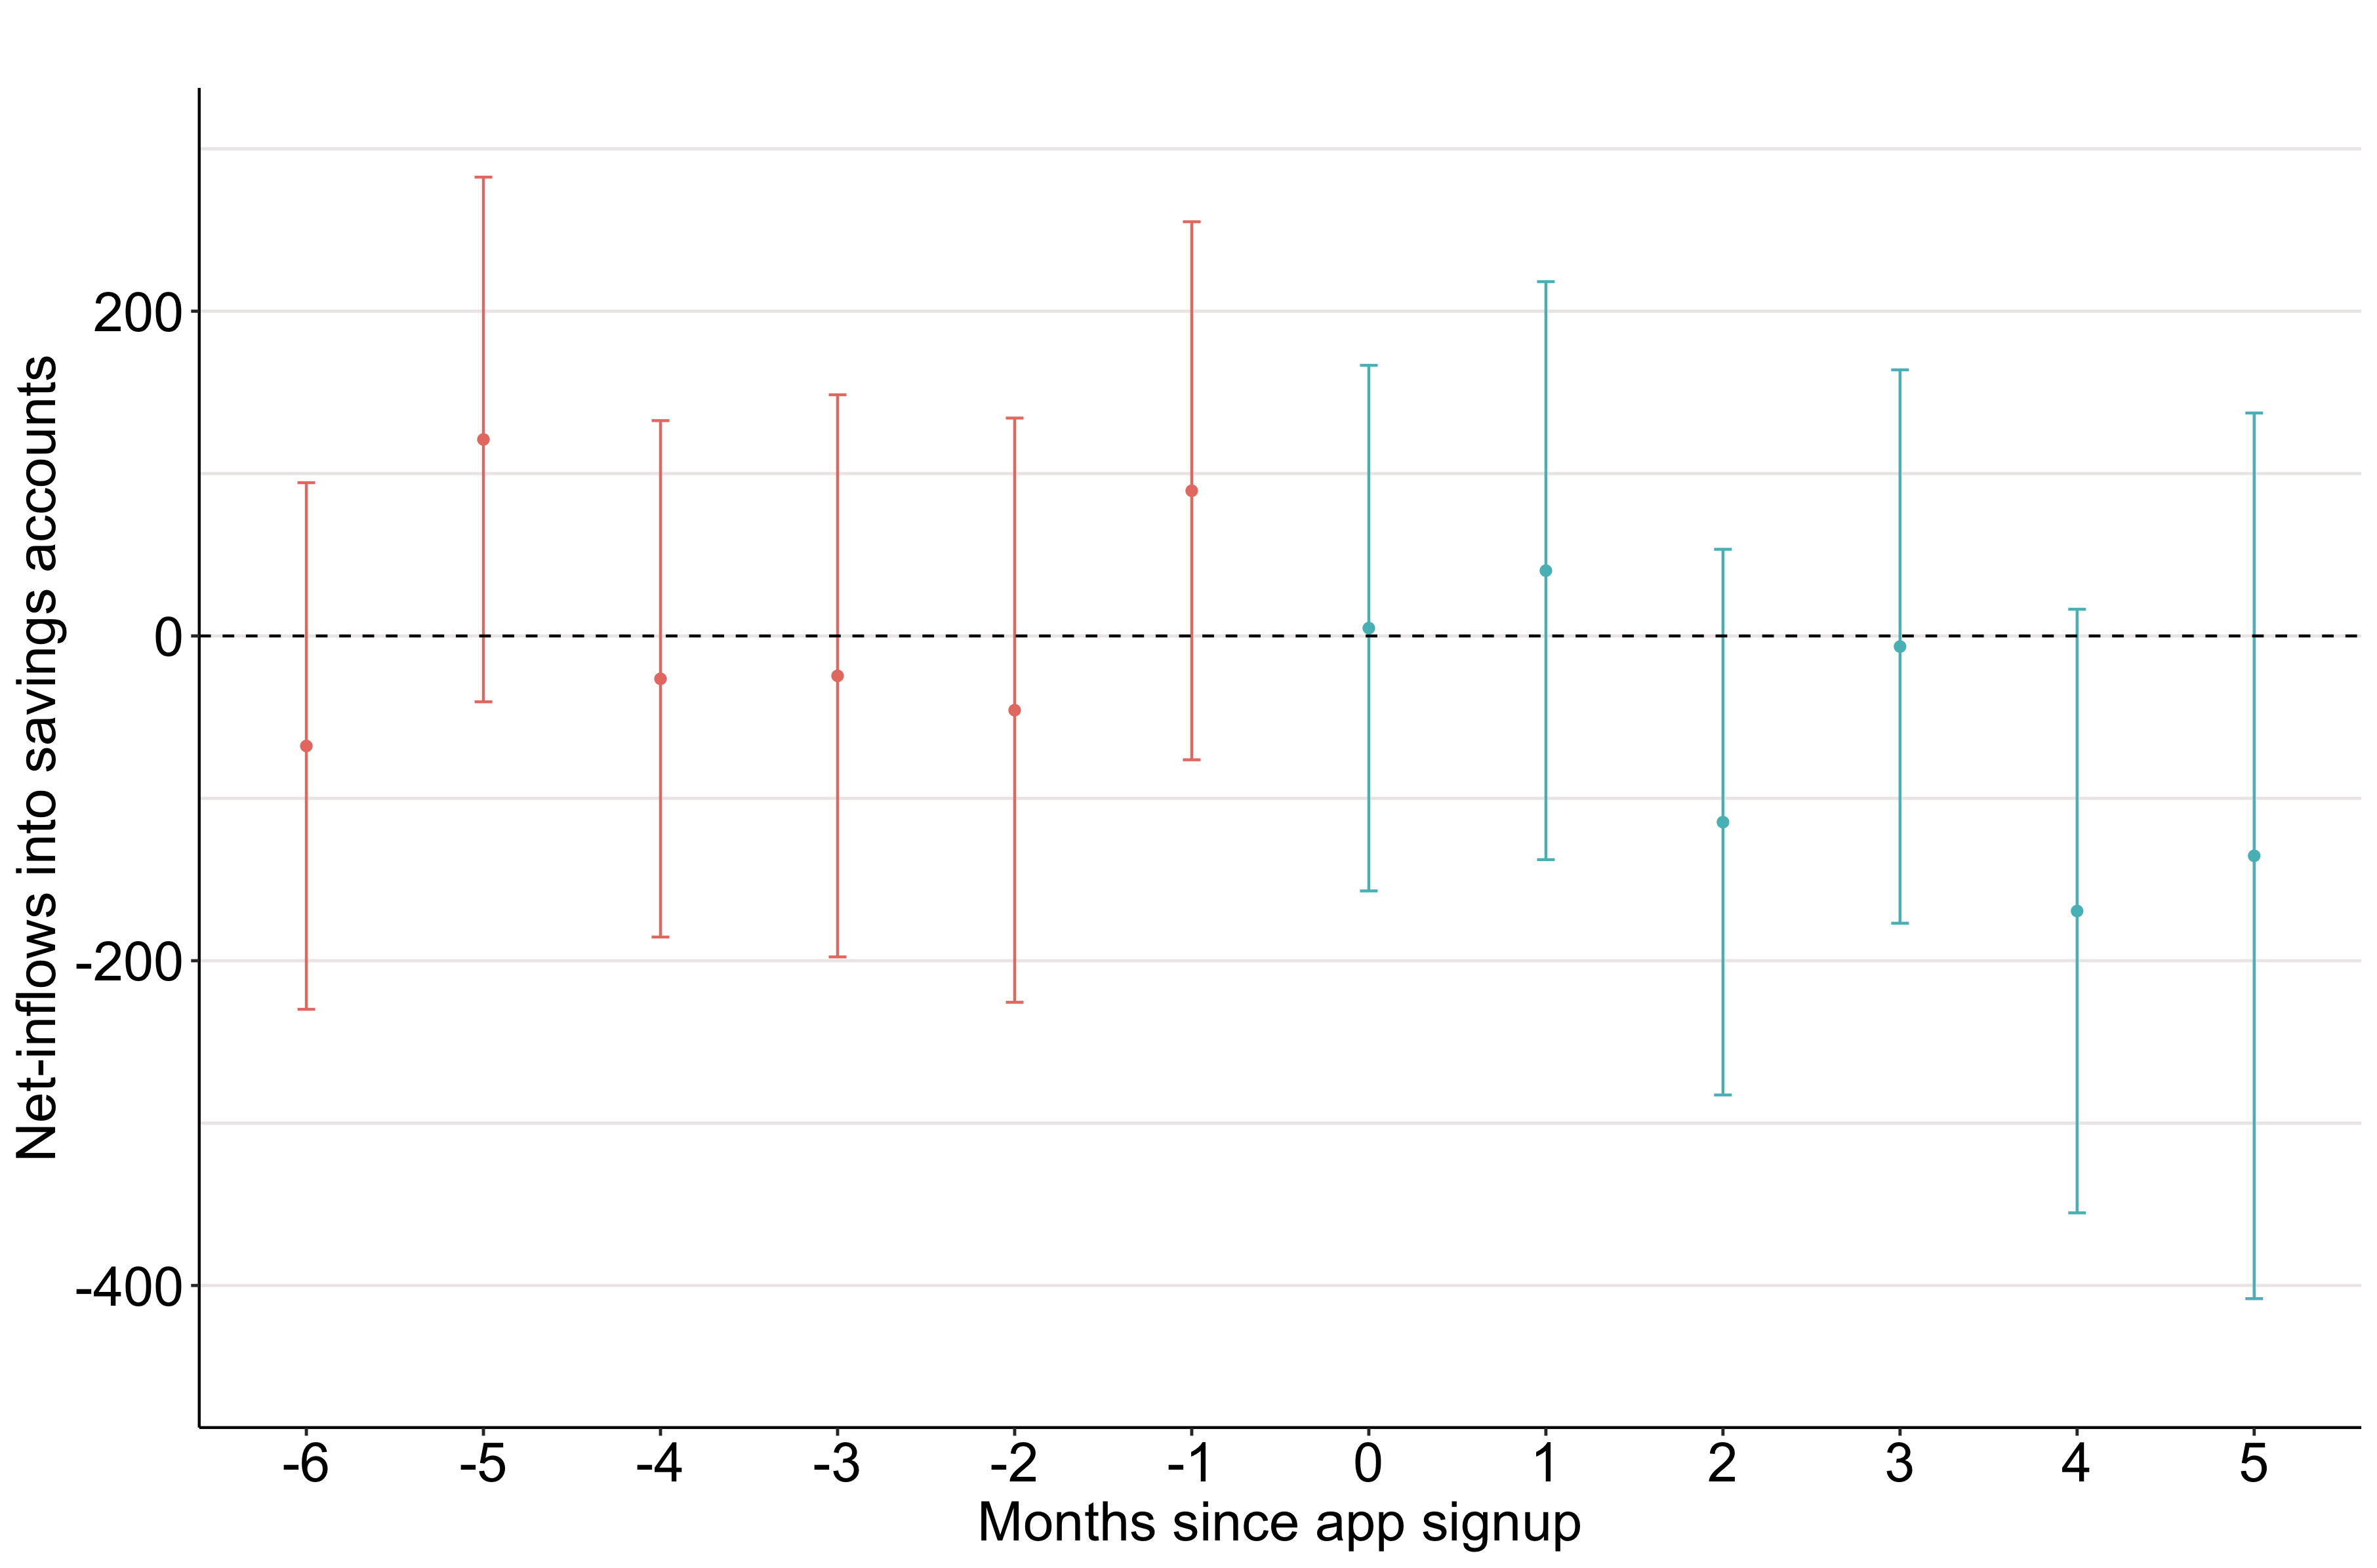
\includegraphics[width=.49\textwidth]{\figdir/netflows_cond_es.png}
    \fignote{\textwidth}{The effect of app use on monthly discretionary
        spending (top row) and monthly net-inflows into savings accounts
        (bottom row) under the unconditional (left column) and conditional
        (right column) parallel trends assumption. Point estimates represent
        group-time average treatment effects aggregated to periods since
        treatment exposure, as defined in Section~\ref{sec:estimation}. Red
        lines represent point estimates and uniform 95\% confidence bands for
        pre-treatment periods allowing for clustering at the user level. If the
        null hypothesis that parallel trends hold in all periods is correct,
        these should be equal to zero. Blue lines provide similar information
    for post-treatment periods.}
\end{figure}

Figure~\ref{fig:main_results} shows the effect of app use on monthly
discretionary spend (top row) and monthly net-inflows into savings accounts
(bottom row) under the unconditional (left column) and conditional (right
column) parallel trends assumptions. As discussed in
Section~\ref{sec:estimation}, the conditional parallel trends assumption states
that the outcome variable of treatment and control units with the same set of
covariates would have evolved in parallel fashion. Throughout my analysis, the
set of covariates I use are month income, month spend, the number of active
accounts, and age. Estimates are group-time average treatment effects
aggregated by time since treatment exposure, as defined in
Equation~\ref{eq:att_es}. All results are presented with a uniform 95\%
confidence band, based on bootstrapped standard errors that account for
autocorrelation in the data and are clustered at the user level, as discussed
in Section~\ref{sec:estimation}.

We can see that discretionary spend falls by between \pounds100 and \pounds150
per month once users start using the app, depending on the parallel trends
assumption used. Given that average monthly discretionary spend is about
\pounds860 (see Table~\ref{tab:sumstats}), this corresponds to a drop in
discretionary spend of about 11-17 percent, which is substantial. These results
are in line with those found in \citet{levi2020mind}, which find a 11.6 percent
reduction in discretionary spend following the use of an aggregator app.
Interestingly, we can also see that at least for the first six months of app
use, the effect is persistent.

That the results based on the unconditional and the conditional parallel trends
assumptions are very similar but not identical is not surprising. Conditional
parallel trends are important in contexts when (i) there are covariate specific
trends in outcome paths and (ii) the distribution of covariates differs between
treatment and control groups. A classic example of the latter would be
comparing individuals who did and did not sign up for a job-training program,
where characteristics such as age and employment history are often quite
different \citep{heckman1997matching}. In our context, however, where all
individuals eventually sign up to Money Dashboard and our comparison group is a
set of ``not-yet-treated'' rather than ``never-treated'' individuals, we would
not expect covariate values between individuals in the treatment and control
groups to vary as much. At the same time, we would expect the results to differ
somewhat. If, as is plausible, discretionary spend is a constant fraction of
income and total spend, then we would expect parallel trends only for
individuals with similar incomes and total spend. Similarly, if we think that
discretionary spend increases in the number of accounts we observe per user,
then parallel trends in spend only holds for users for whom we observe the same
number of accounts.\footnote{As discussed in Section~\ref{sec:data}, users
    choose which accounts to link to Money Dashboard, and while I select for
    users that appear to have linked all their accounts and for whom we could
    observe the complete account history even if they added some of their
accounts after joining, I cannot rule out that some users do add account after
signup and MDB is unable to capture the complete history.}

We can also see that in two periods, the null-hypothesis of identical
pre-signup trends is being rejected (both under conditional and unconditional
trends). The estimated differences from zero are not large, but a sign that the
results should be interpreted with caution. In future work, I plan to use the
approach introduced by \citet{rambachan2022more} to test how sensitive my
results are to deviations from parallel trends.

Finally, we can see that, in contrast to discretionary spending, net-inflows
into savings accounts do not change once users start using the app. This is
somewhat surprising, since we might have expected that users transfer at least
some of their saved funds into their savings accounts to either build up a
emergency savings cushion or as a contribution towards specific savings goals.
The absence of such transfers naturally begs the question ``where does the
money go?'', to which I turn in the next section.


\subsection{Where do additional funds go?}%
\label{sub:where_do_additional_funds_go_}

Above, we found that while users reduce their discretionary spend after using
MDB by between \pounds100 and \pounds150, they do not transfer additional funds
into their savings accounts.

One possible explanation is that users do save more but transfer money either
into longer-term savings vehicles such as investment funds or into savings
accounts they have not linked to MDB. The first three panels (from the top
left) in Figure~\ref{fig:wdmg} show flows into investment of pension funds,
current account outflows that users manually labelled as ``savings'', and -- as
an alternative but cruder measure of transfers into savings accounts -- the
total amount of transfers from current accounts into other accounts held by the
user.\footnote{The code where these variables are defined is available on
\href{https://github.com/fabiangunzinger/mdb_eval/blob/f31bfcd7a330188cdd27968d41957ebf5b454099/src/data/aggregators.py\#L300}{Github}.}
None of these change significantly during users' pre and post signup periods,
rejecting the idea that users systematically move additional funds into either
investment vehicles or other savings accounts. An exception is the spikes in
user-labelled savings in the month just before and the month of signup. Rather
than suggesting an additional inflow of funds, however, this is is more likely
to be an artefact of users only manually labelling transactions during active
app use rather than also labelling historical transactions.\footnote{The pattern
    could be explained in two ways: either users can see the entire account
    history available to MDB after linking an account but only label
    transactions during periods of active app use and the period immediately
before signup, or MDB only shows users data from the month before signup
onwards, so that users are unable to manually label transactions in earlier
periods.}

\begin{figure}[h]
    \centering
    \caption{Possible destinations of additional savings}%
    \label{fig:wdmg}
    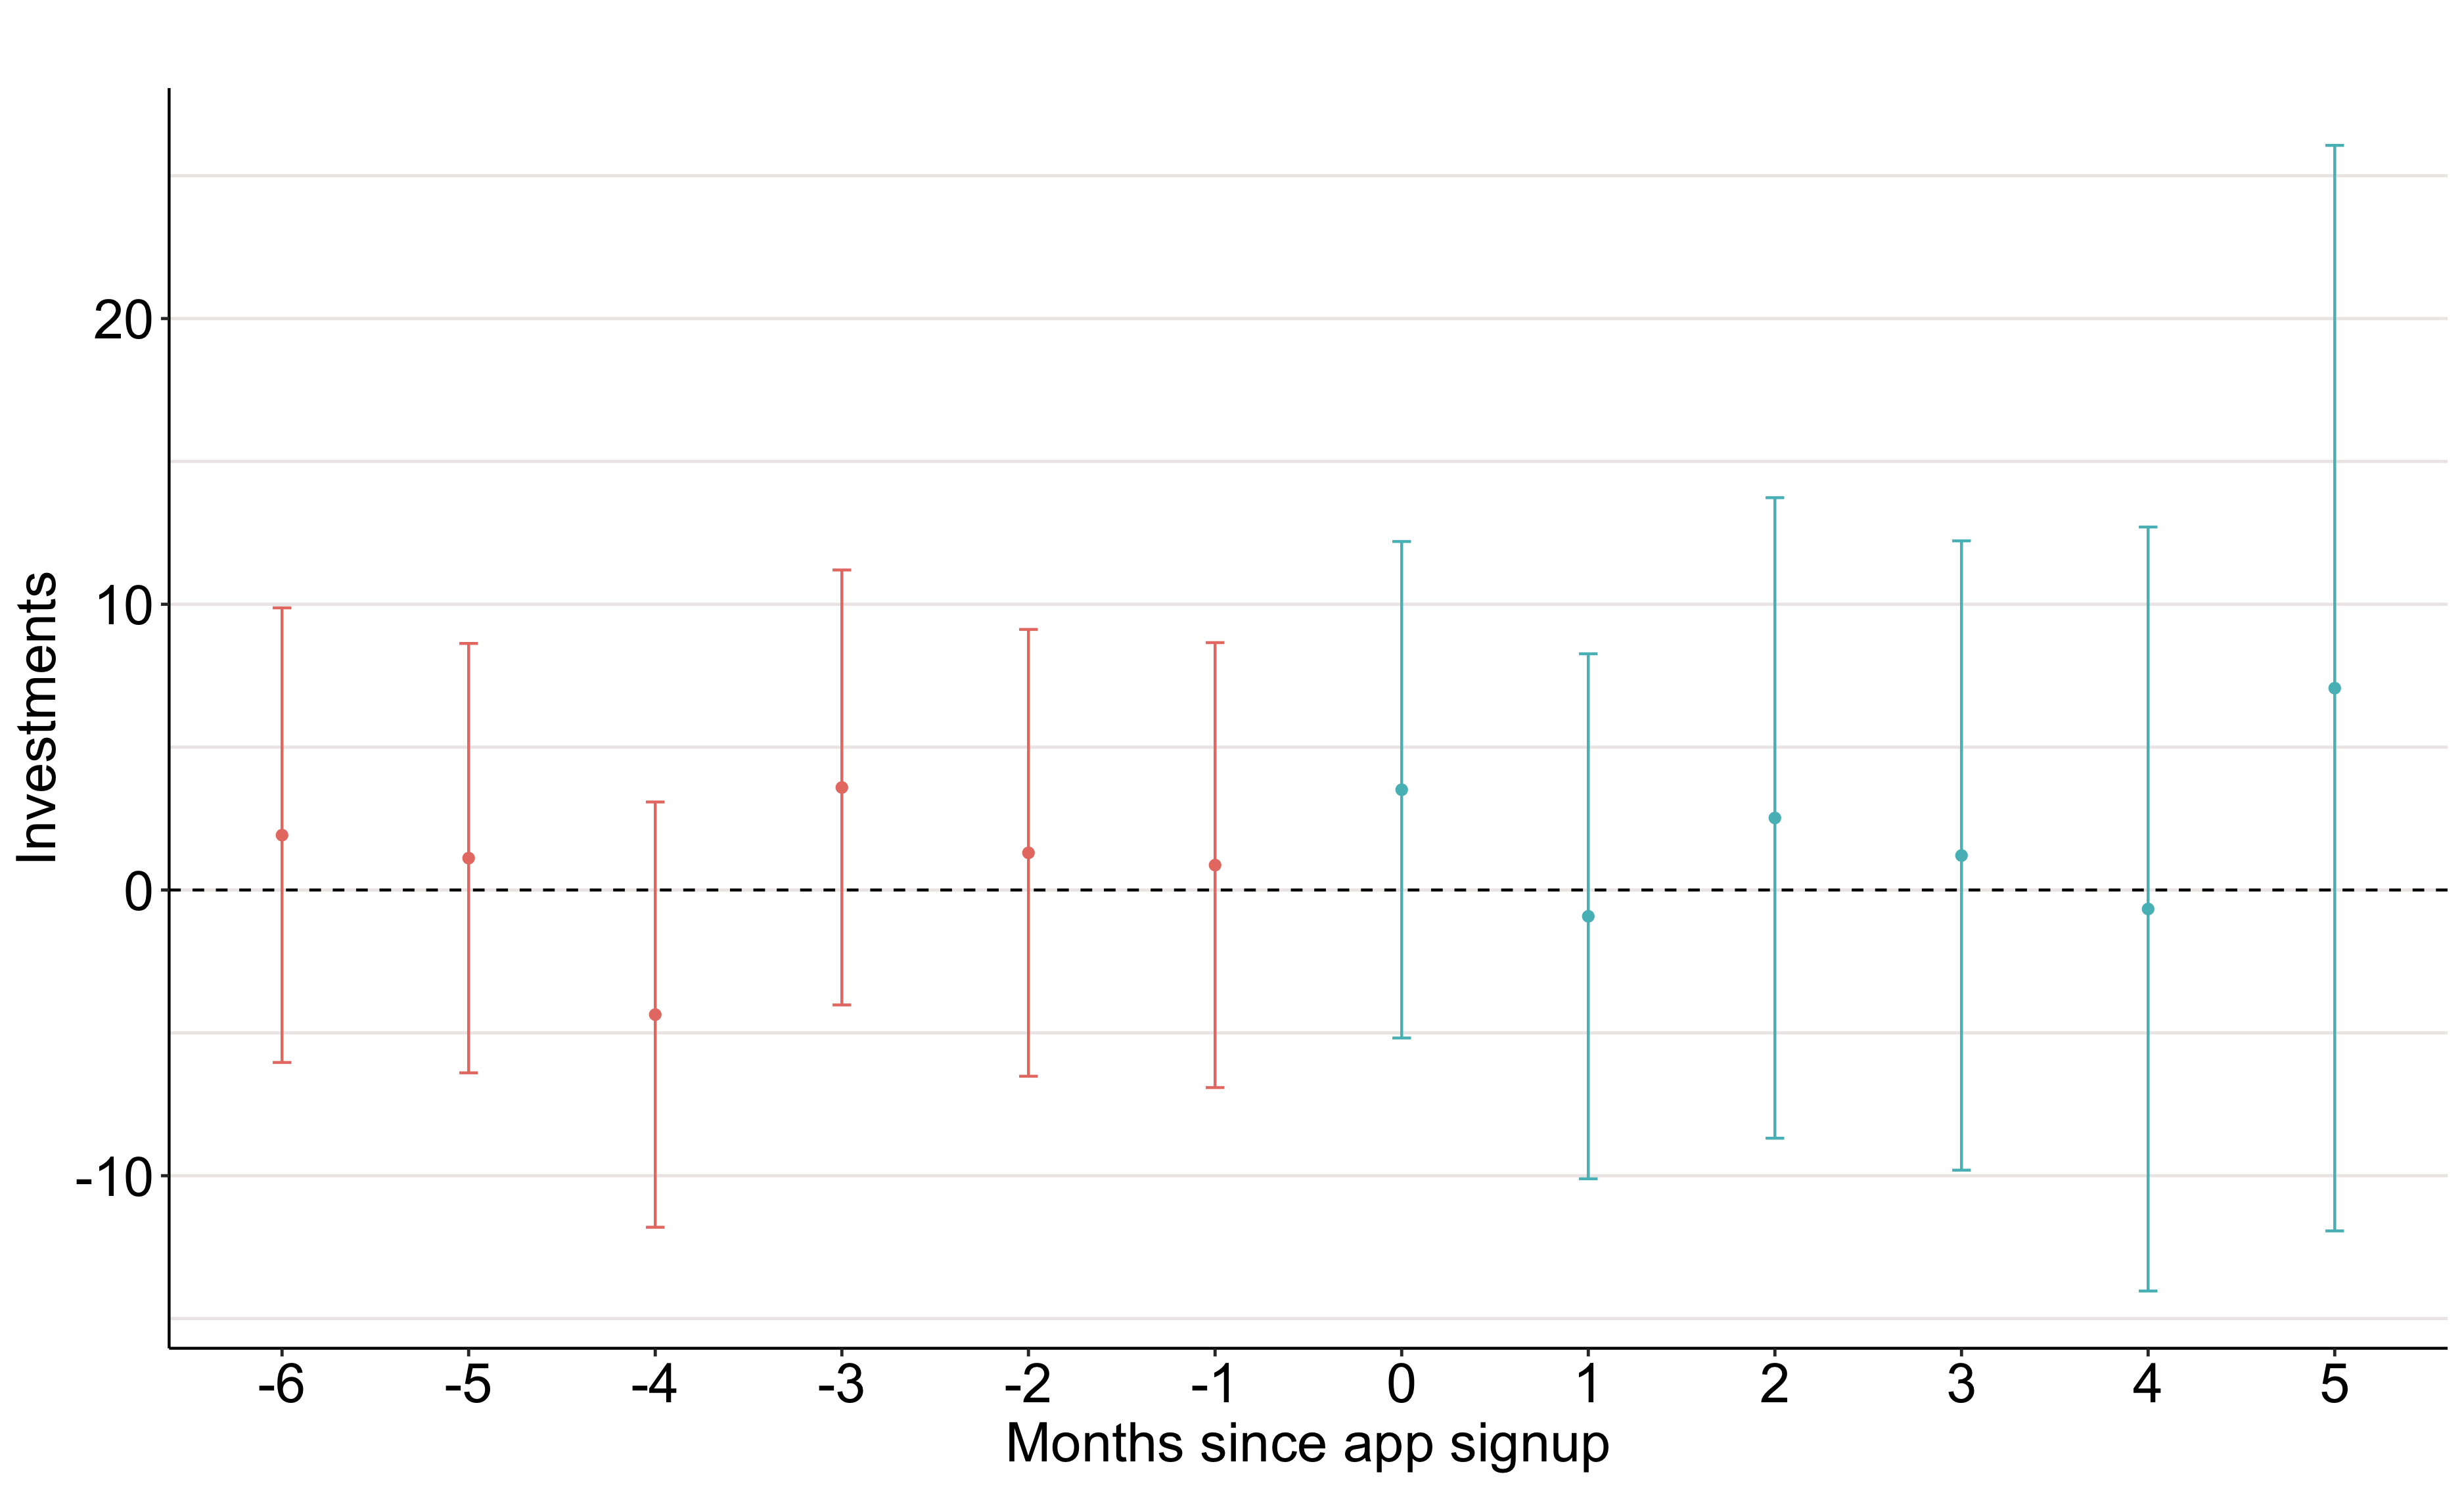
\includegraphics[width=.49\textwidth]{\figdir/investments_cond_es.png}
    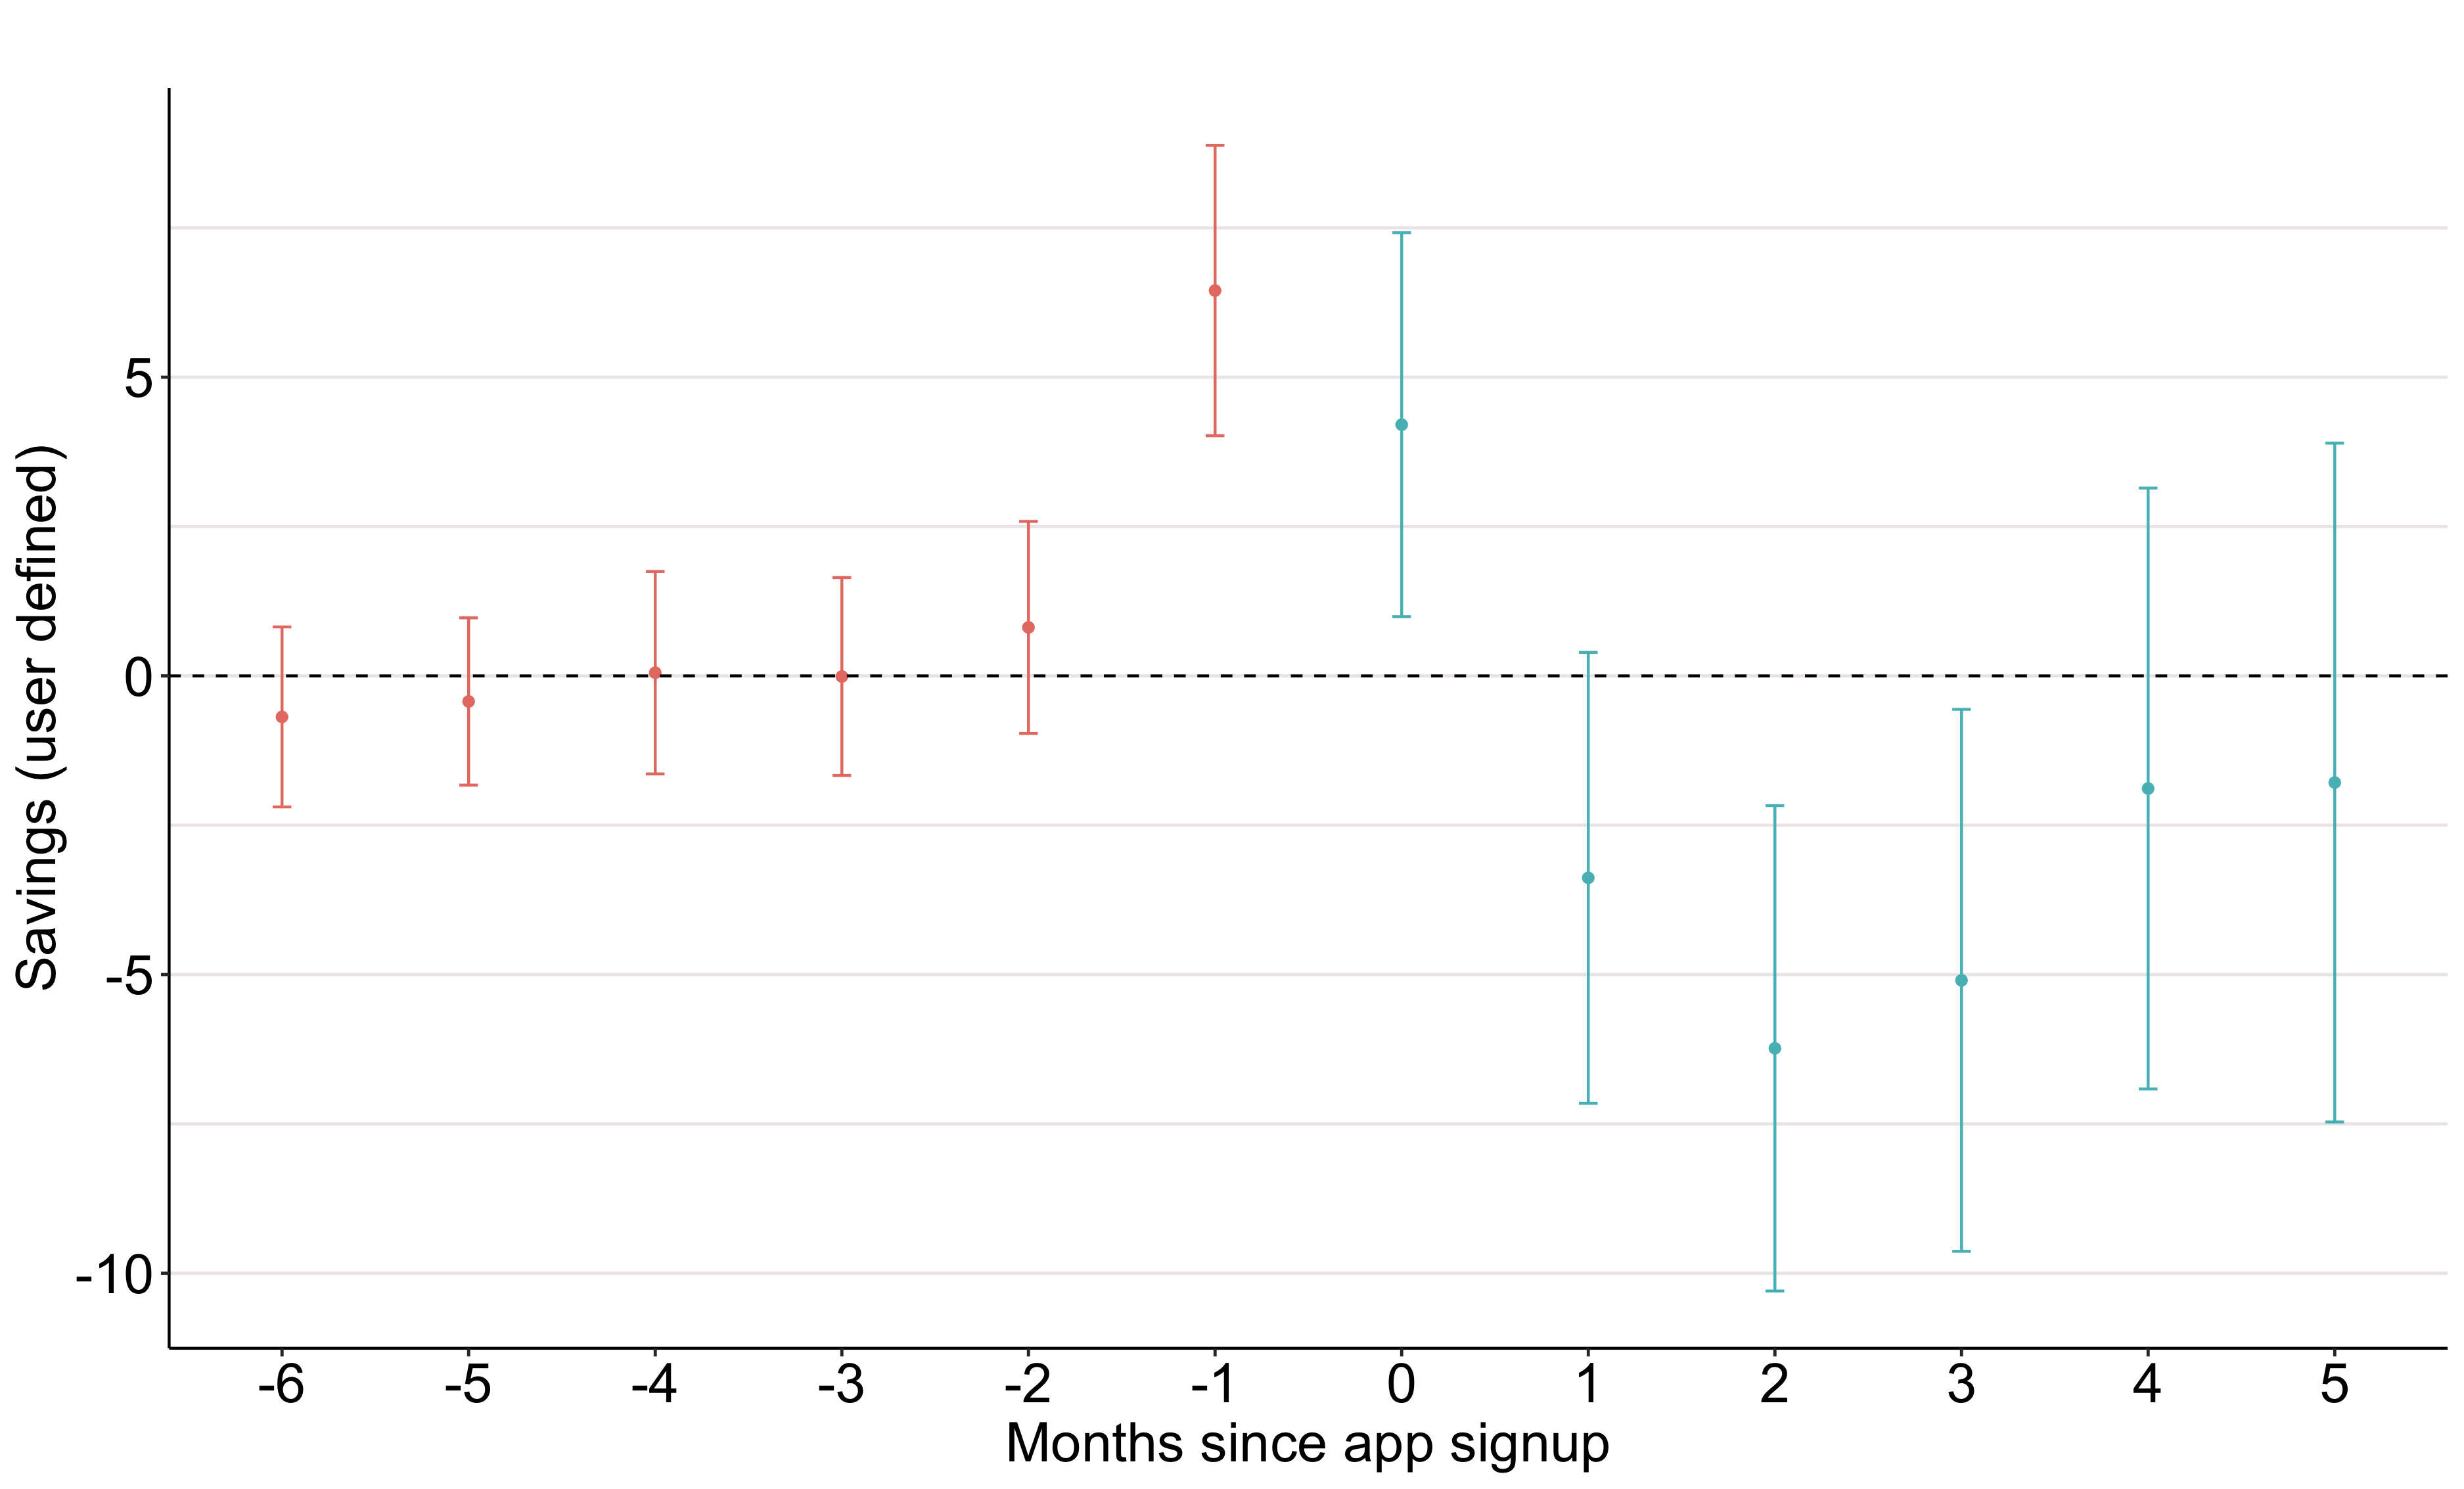
\includegraphics[width=.49\textwidth]{\figdir/up_savings_cond_es.png}
    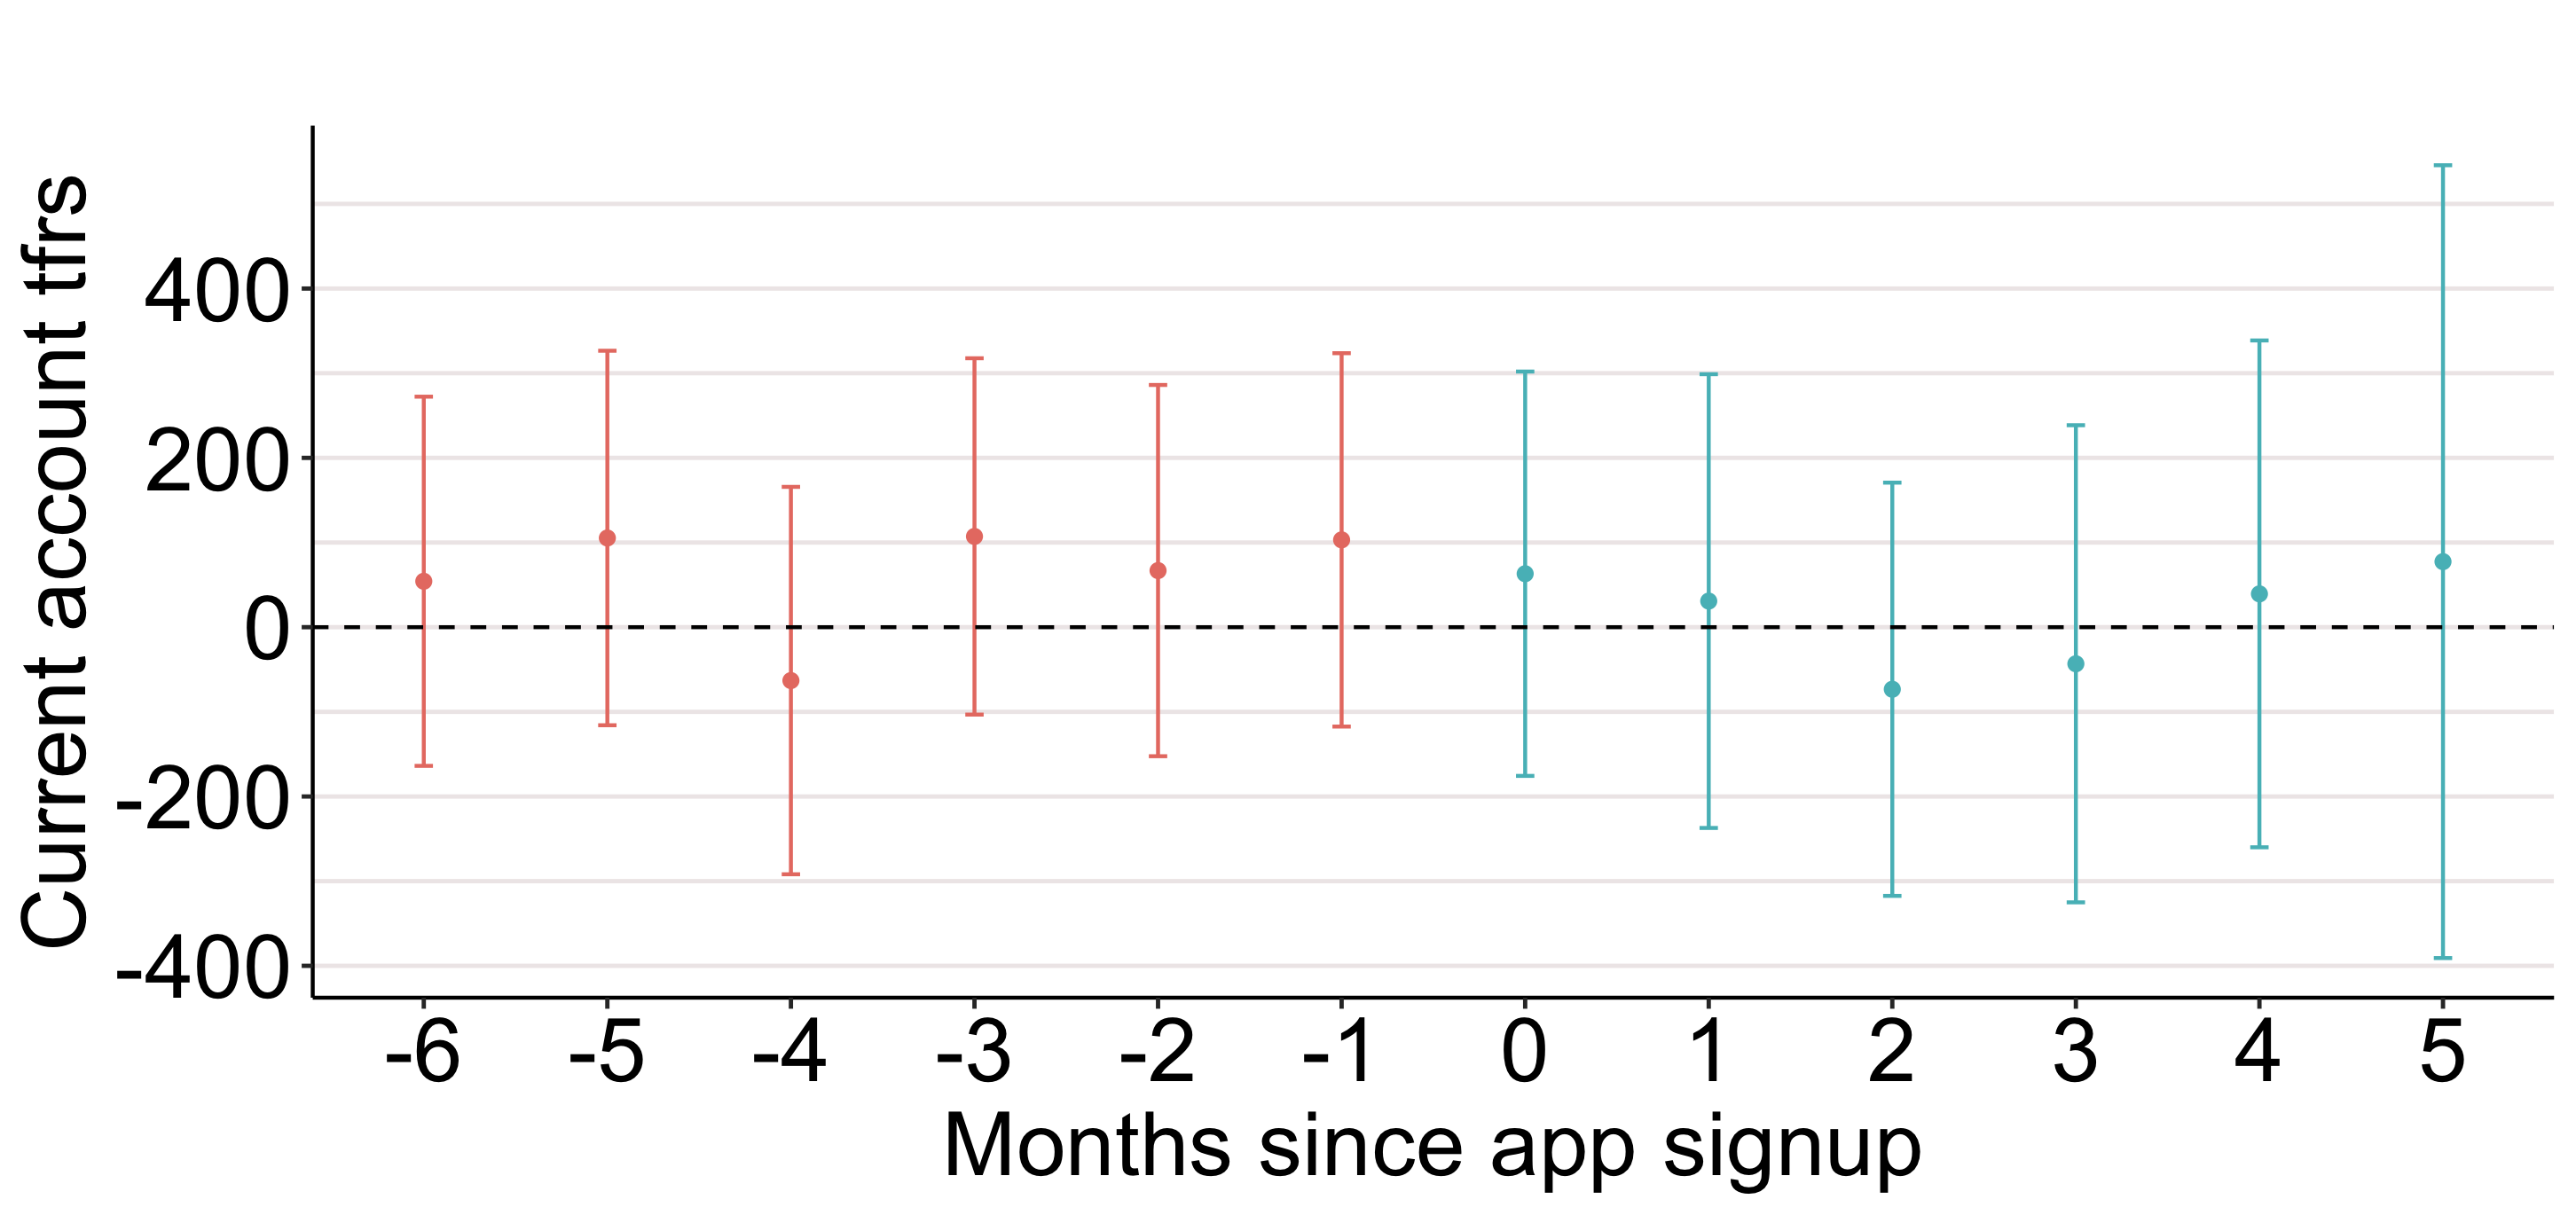
\includegraphics[width=.49\textwidth]{\figdir/ca_transfers_cond_es.png}
    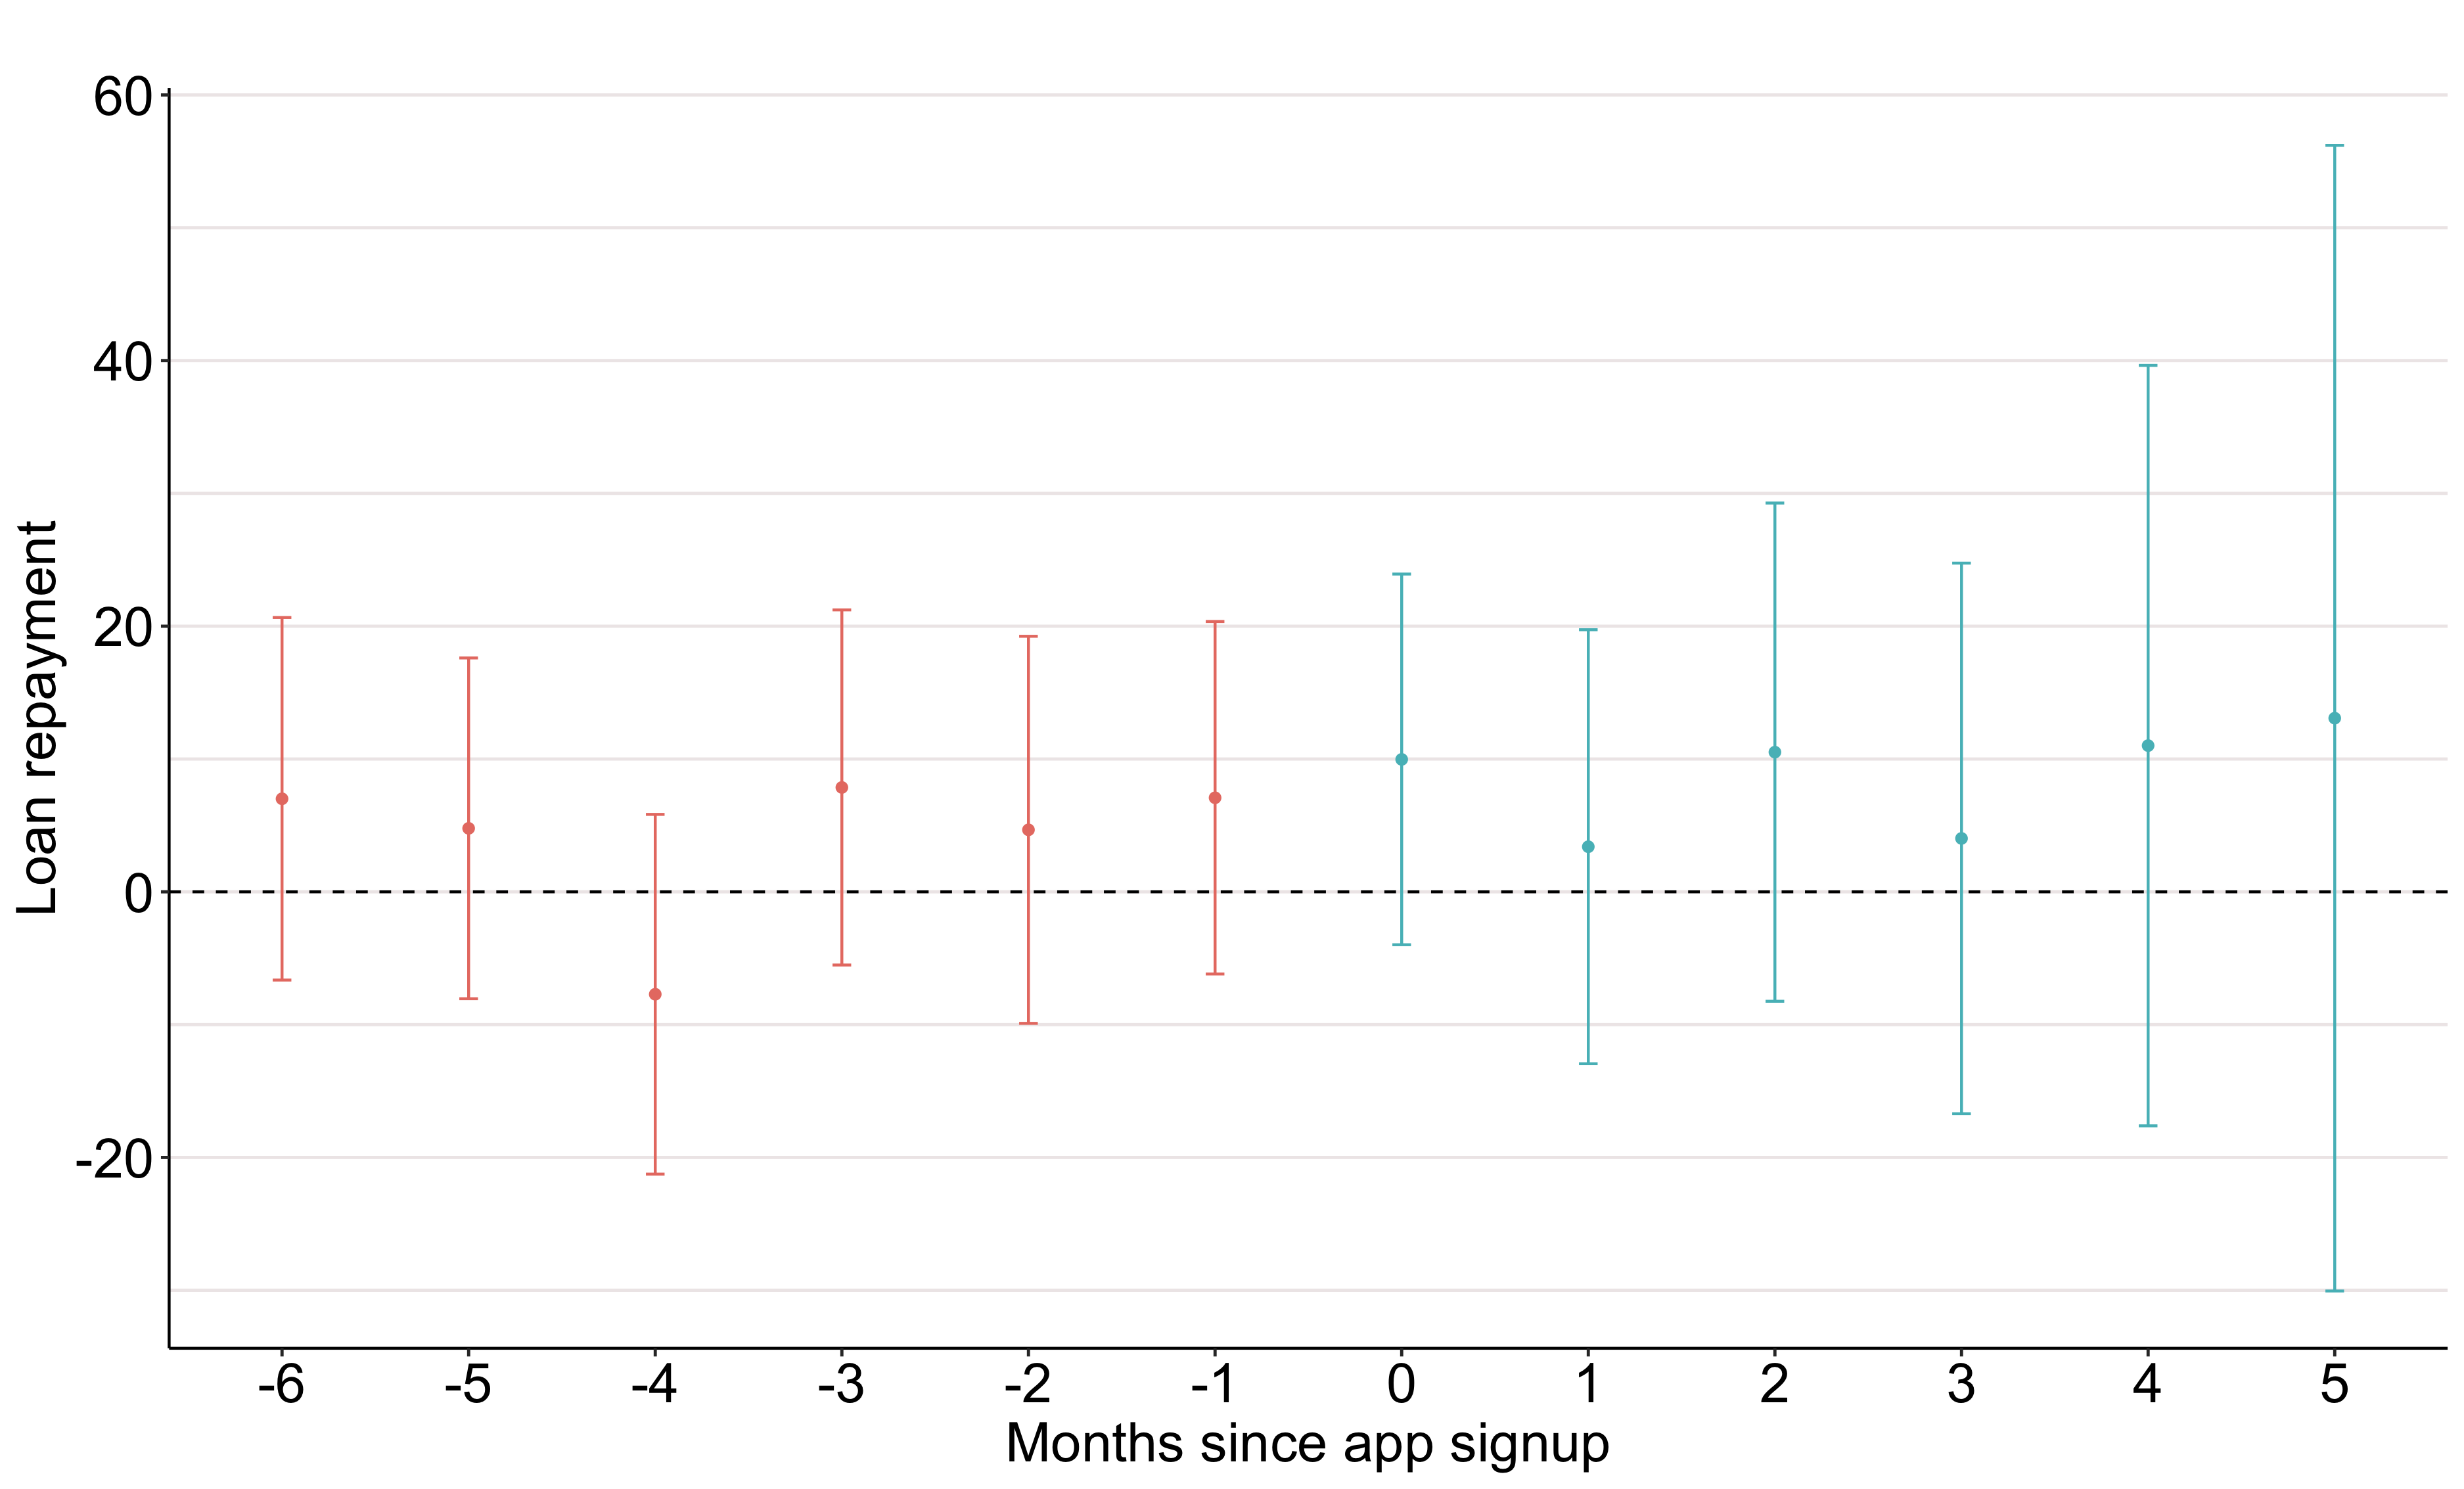
\includegraphics[width=.49\textwidth]{\figdir/loan_rpmts_cond_es.png}
    \fignote{\textwidth}{Point estimates represent
        group-time average treatment effects aggregated to periods since
        treatment exposure, as defined in Section~\ref{sec:estimation}. Red
        lines represent point estimates and uniform 95\% confidence bands for
        pre-treatment periods allowing for clustering at the user level. If the
        null hypothesis that parallel trends hold in all periods is correct,
        these should be equal to zero. Blue lines provide similar information
    for post-treatment periods.}
\end{figure}

Another possibility is that users use the additional funds to pay down debt.
The bottom right panel in Figure~\ref{fig:wdmg} shows loan repayments, which do
not change significantly during the 12-month period around app signup either.

The finding that saved funds do not flow into any of the plausible channels can
be explained in three ways (and any combination thereof): (i) users might leave
saved funds in their current accounts, (ii) users are homogenous and allocate
saved funds across a large number of different uses in amounts I am not powered
to detect, (iii) users are heterogeneous and allocate funds across a small
number of uses that differ between users, so that, in the aggregate, I am not
powered to detect these changes either.


\subsection{Disaggregated discretionary spend}%
\label{sub:disaggregated_discretionary_spend}

Another question of interest based on the main findings above is along what
dimensions users reduce their discretionary spend. There are three dimensions of
interest.

\begin{figure}[h]
    \centering
    \caption{Change in direct-debit discretionary spend}%
    \label{fig:disagg_dd}
    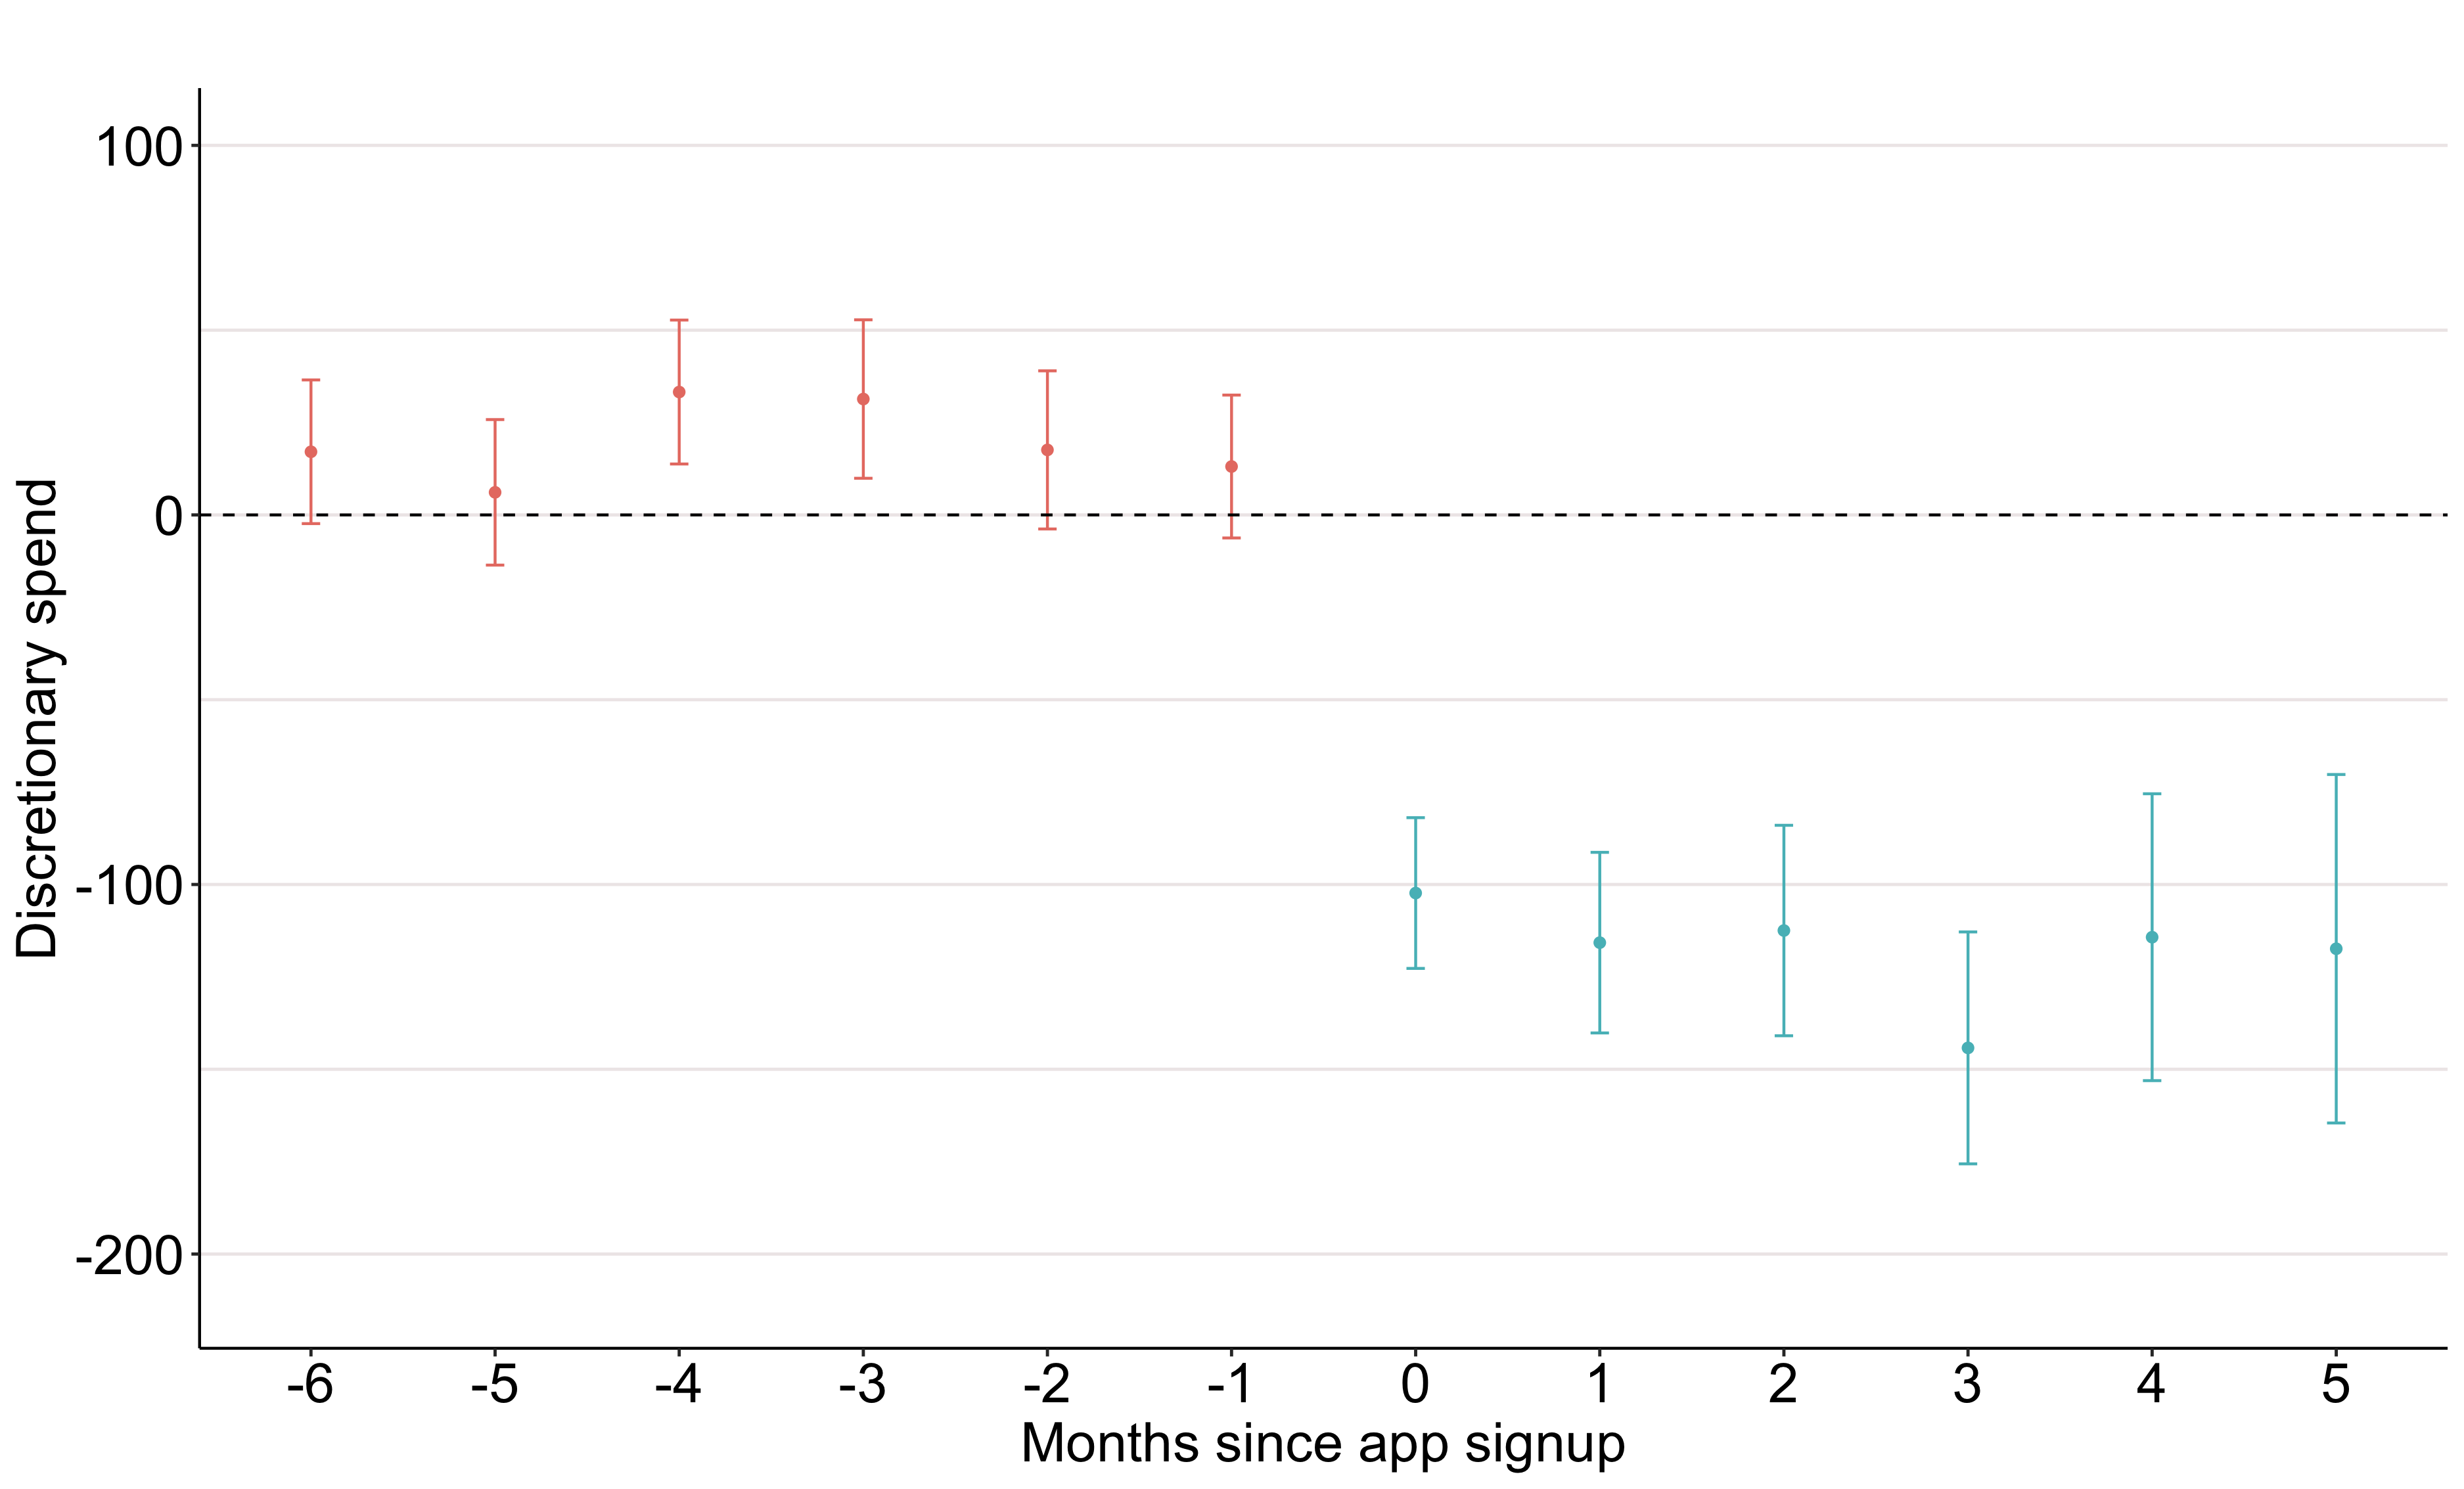
\includegraphics[width=.49\textwidth]{\figdir/disag_dspend_cond_es.png}
    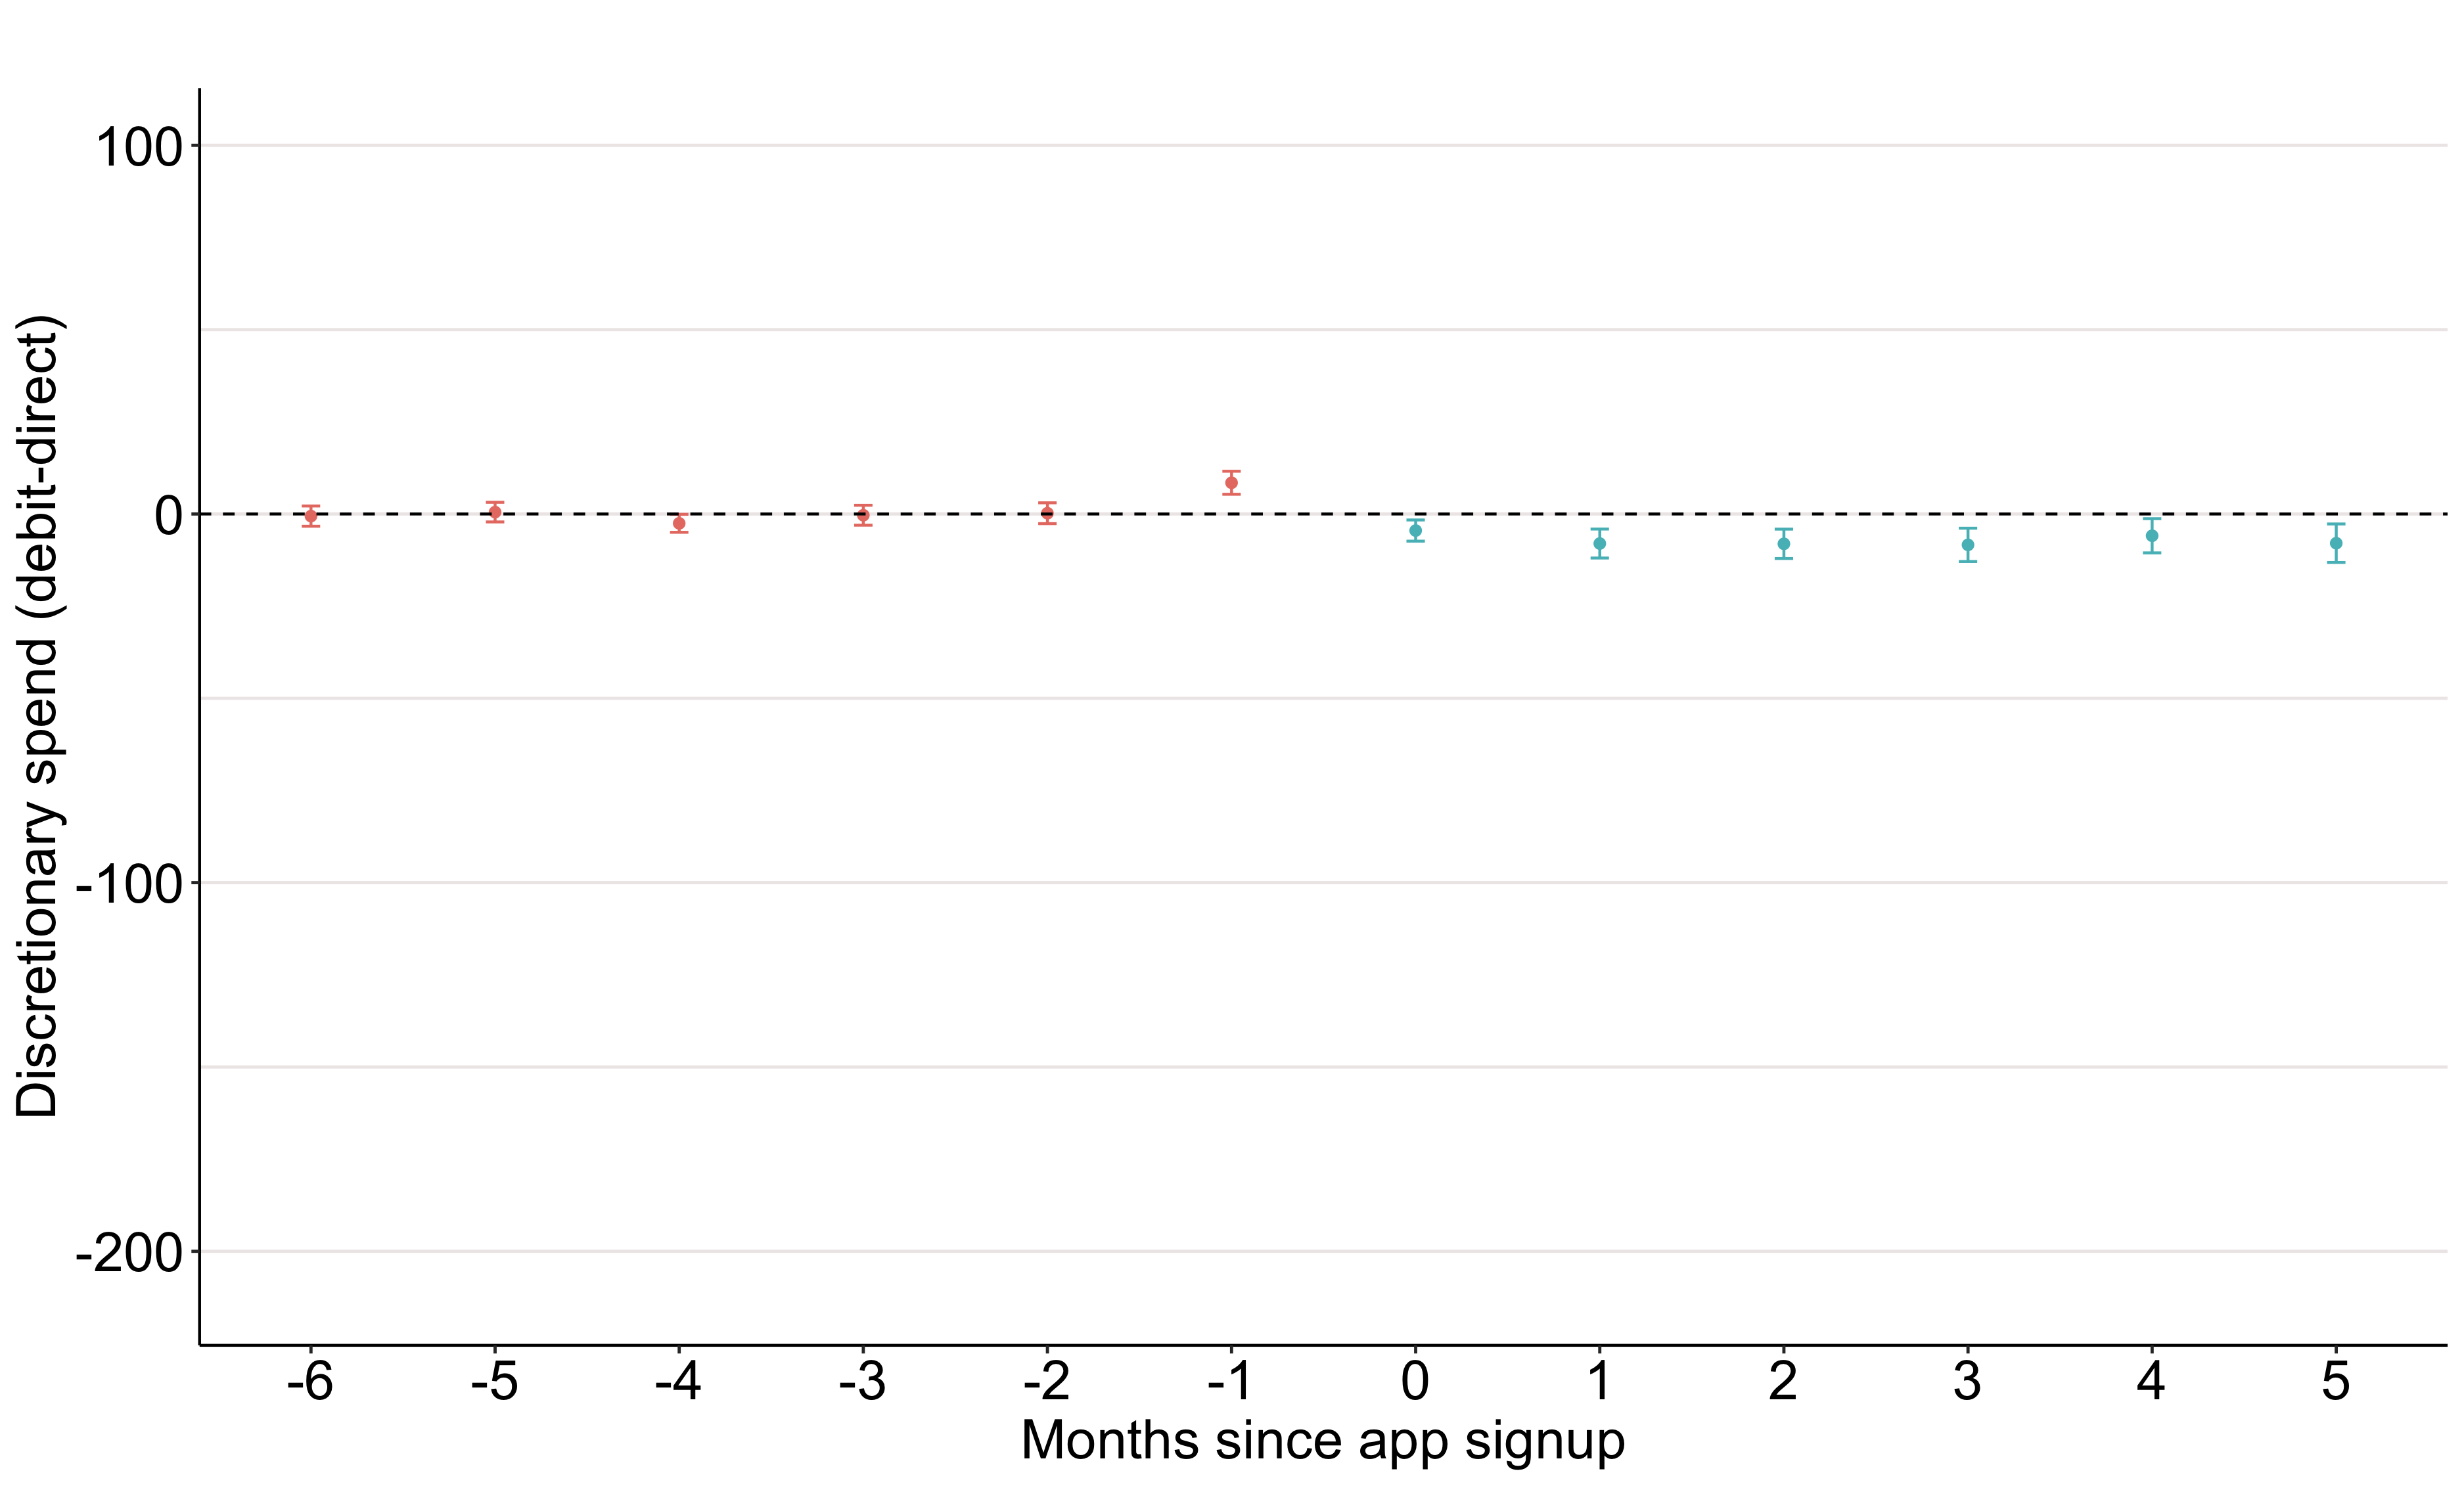
\includegraphics[width=.49\textwidth]{\figdir/disag_dspend_dd_cond_es.png}
    \fignote{\textwidth}{Effect of app use on total discretionary spend (for
        reference) and discretionary spend paid via debit-direct contracts.
        Point estimates represent group-time average treatment effects
        aggregated to periods since treatment exposure, as defined in
        Section~\ref{sec:estimation}. Red lines represent point estimates and
        uniform 95\% confidence bands for pre-treatment periods allowing for
        clustering at the user level. If the null hypothesis that parallel
        trends hold in all periods is correct, these should be equal to zero.
    Blue lines provide similar information for post-treatment periods.}
\end{figure}

First, users can achieve the persistent reduction in discretionary
spend seen in Figure~\ref{fig:main_results} by either maintaining a change in
behaviour consistently month-to-month by, for instance, making fewer purchases
or spending less on certain items, or, alternatively, make a decision during
the month of signup that automates the reduction in spend by cancelling
debit-direct contracts. Figure~\ref{fig:disagg_dd} shows in the left panel the
reduction of discretionary spending shows in Figure~\ref{fig:main_results}
above for reference, and in the right panel discretionary spend paid via
debit-direct contracts. It shows that debit-direct discretionary spend falls
only marginally after app use, indicating that it is a change in behaviour
sustained month-to-month that drives the reduction in discretionary spend. A
caveat to this analysis is that the MDB data allows for only imperfect
identification of debit-direct transactions for two reasons: first, only some
banks label debit-direct transactions as such in the transaction descriptions
provided to MDB and it is commonly applied labels that I use to identify the
transactions. Second, MDB redacts some transaction descriptions entirely or in
part to ensure the anonymity of its users, and its possible that some of these
transactions are debit-directs.\footnote{The code used to calculate
debit-direct discretionary spend is available on
\href{https://github.com/fabiangunzinger/mdb_eval/blob/f31bfcd7a330188cdd27968d41957ebf5b454099/src/data/aggregators.py\#L461}{Github}.}

\begin{figure}[h]
    \centering
    \caption{Change in discretionary spend by subgroup}%
    \label{fig:disagg_groups}
    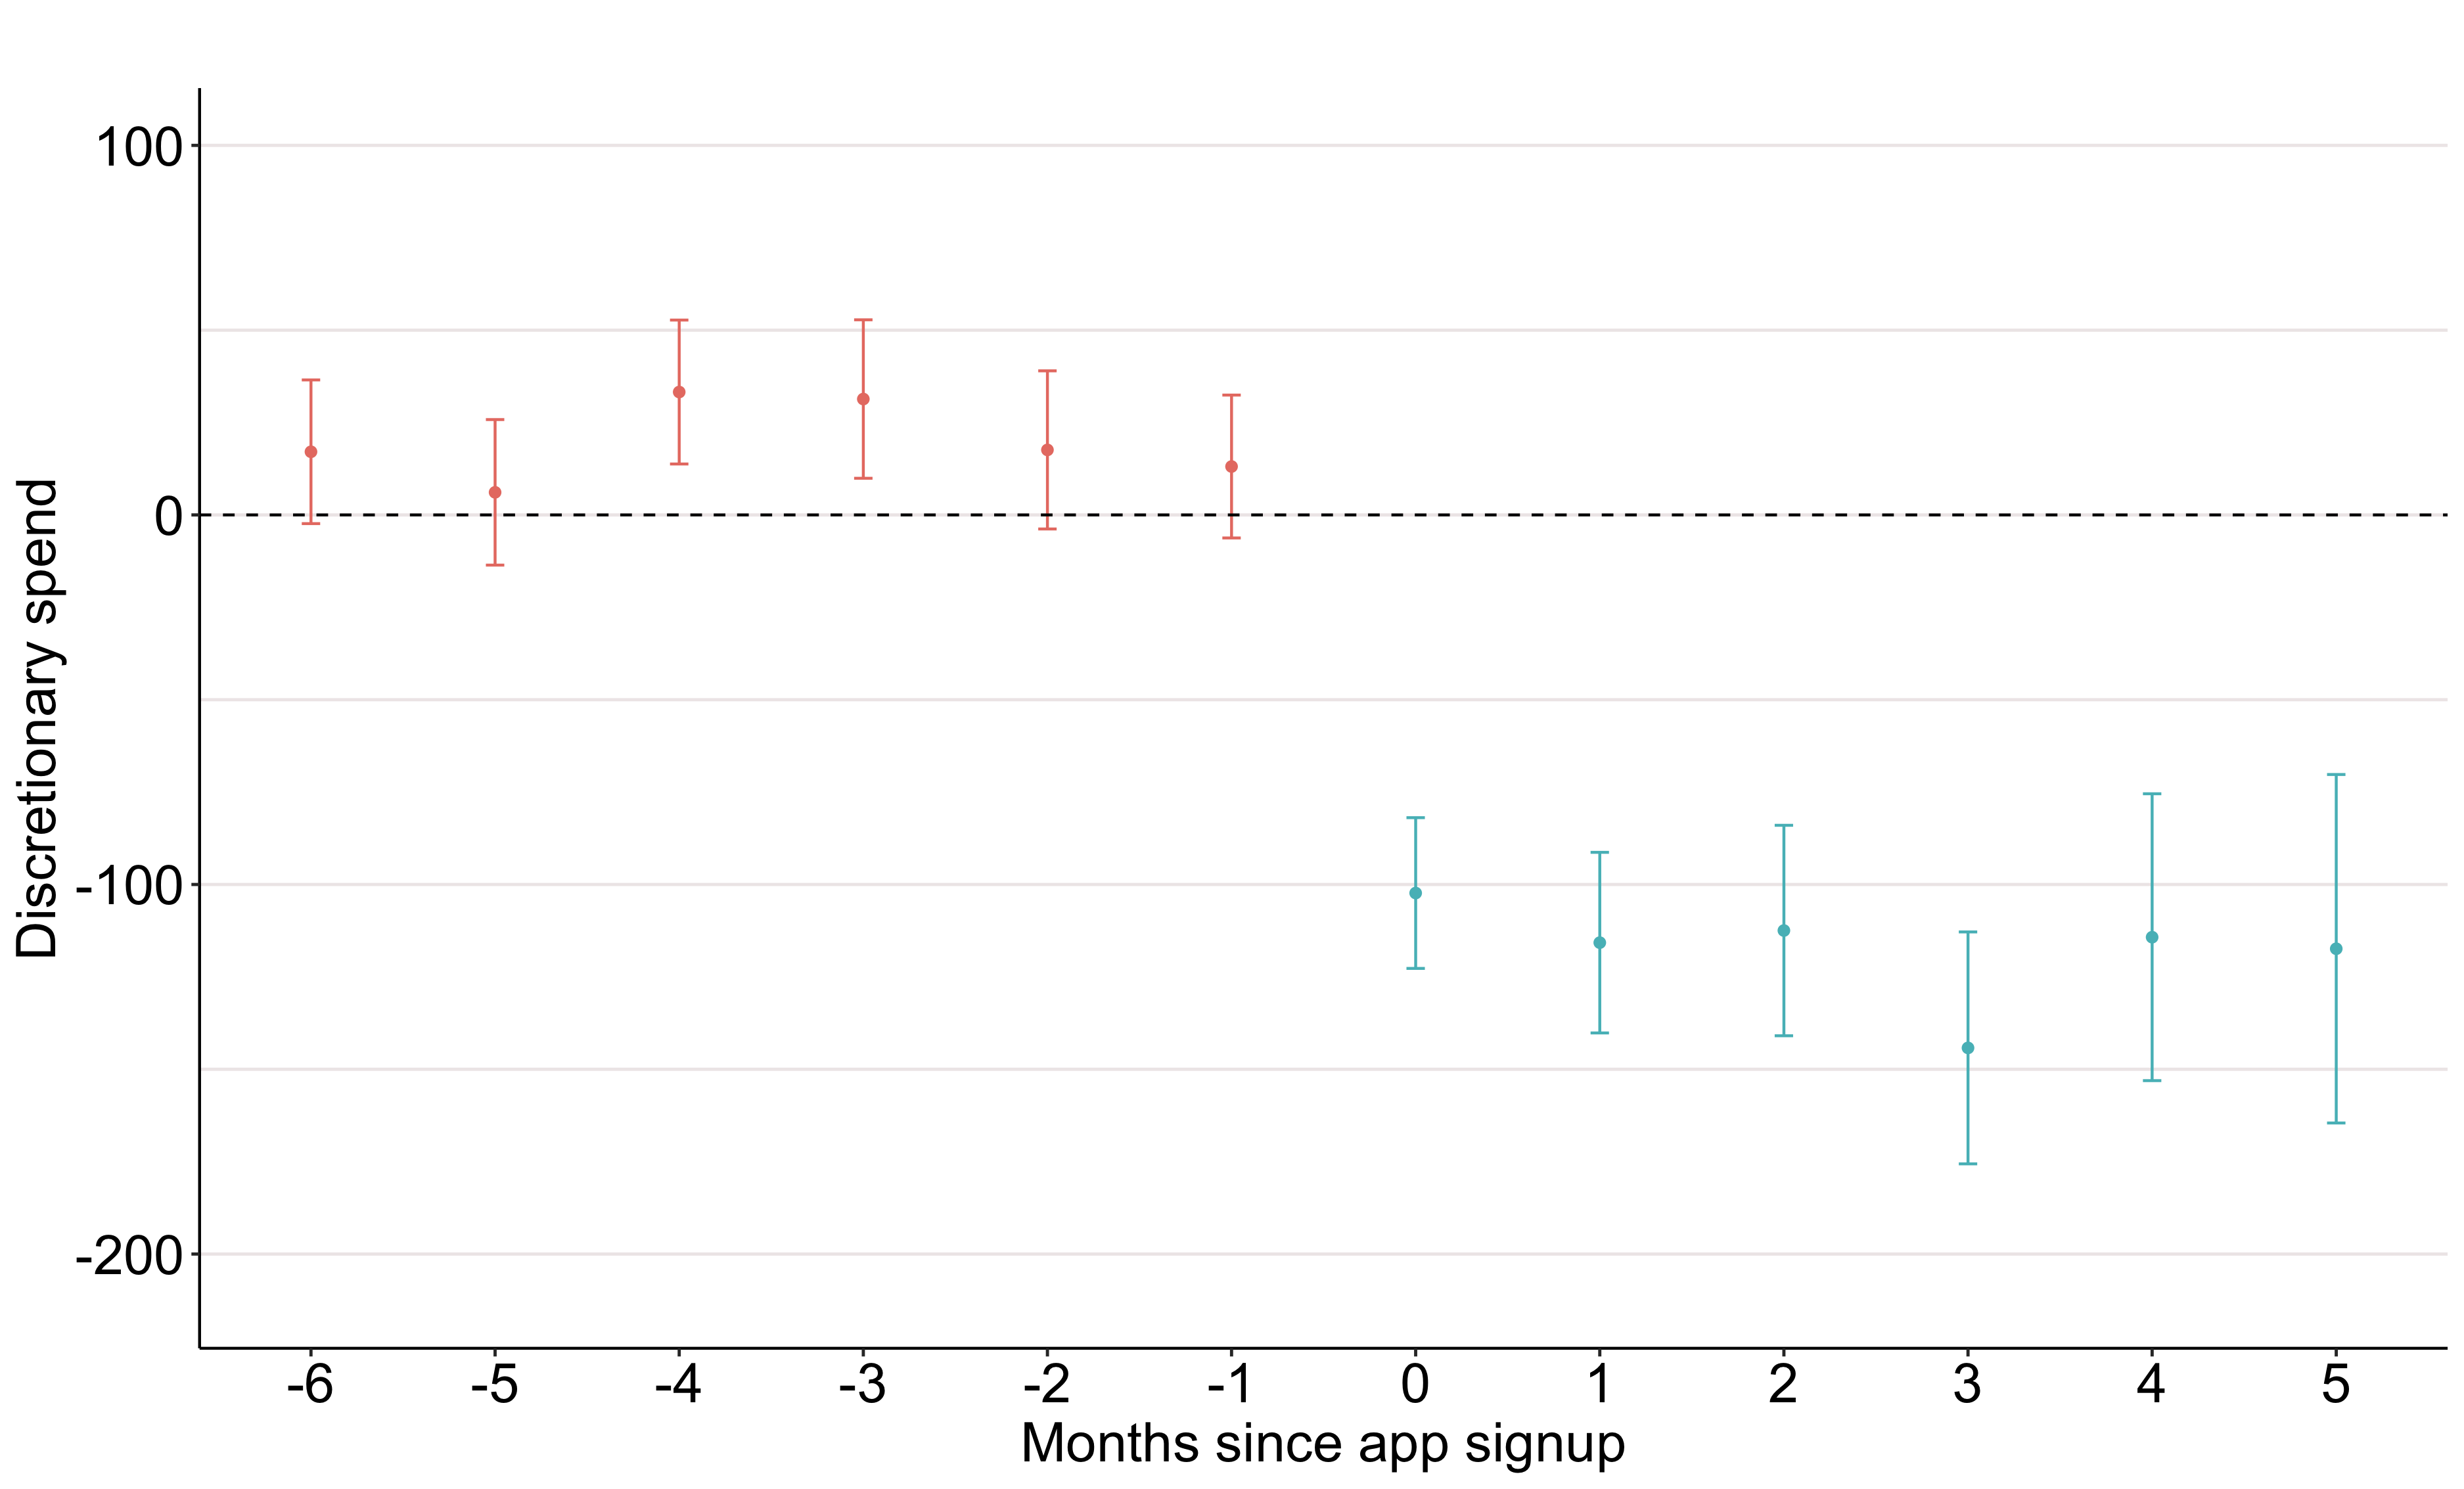
\includegraphics[width=.49\textwidth]{\figdir/disag_dspend_cond_es.png}
    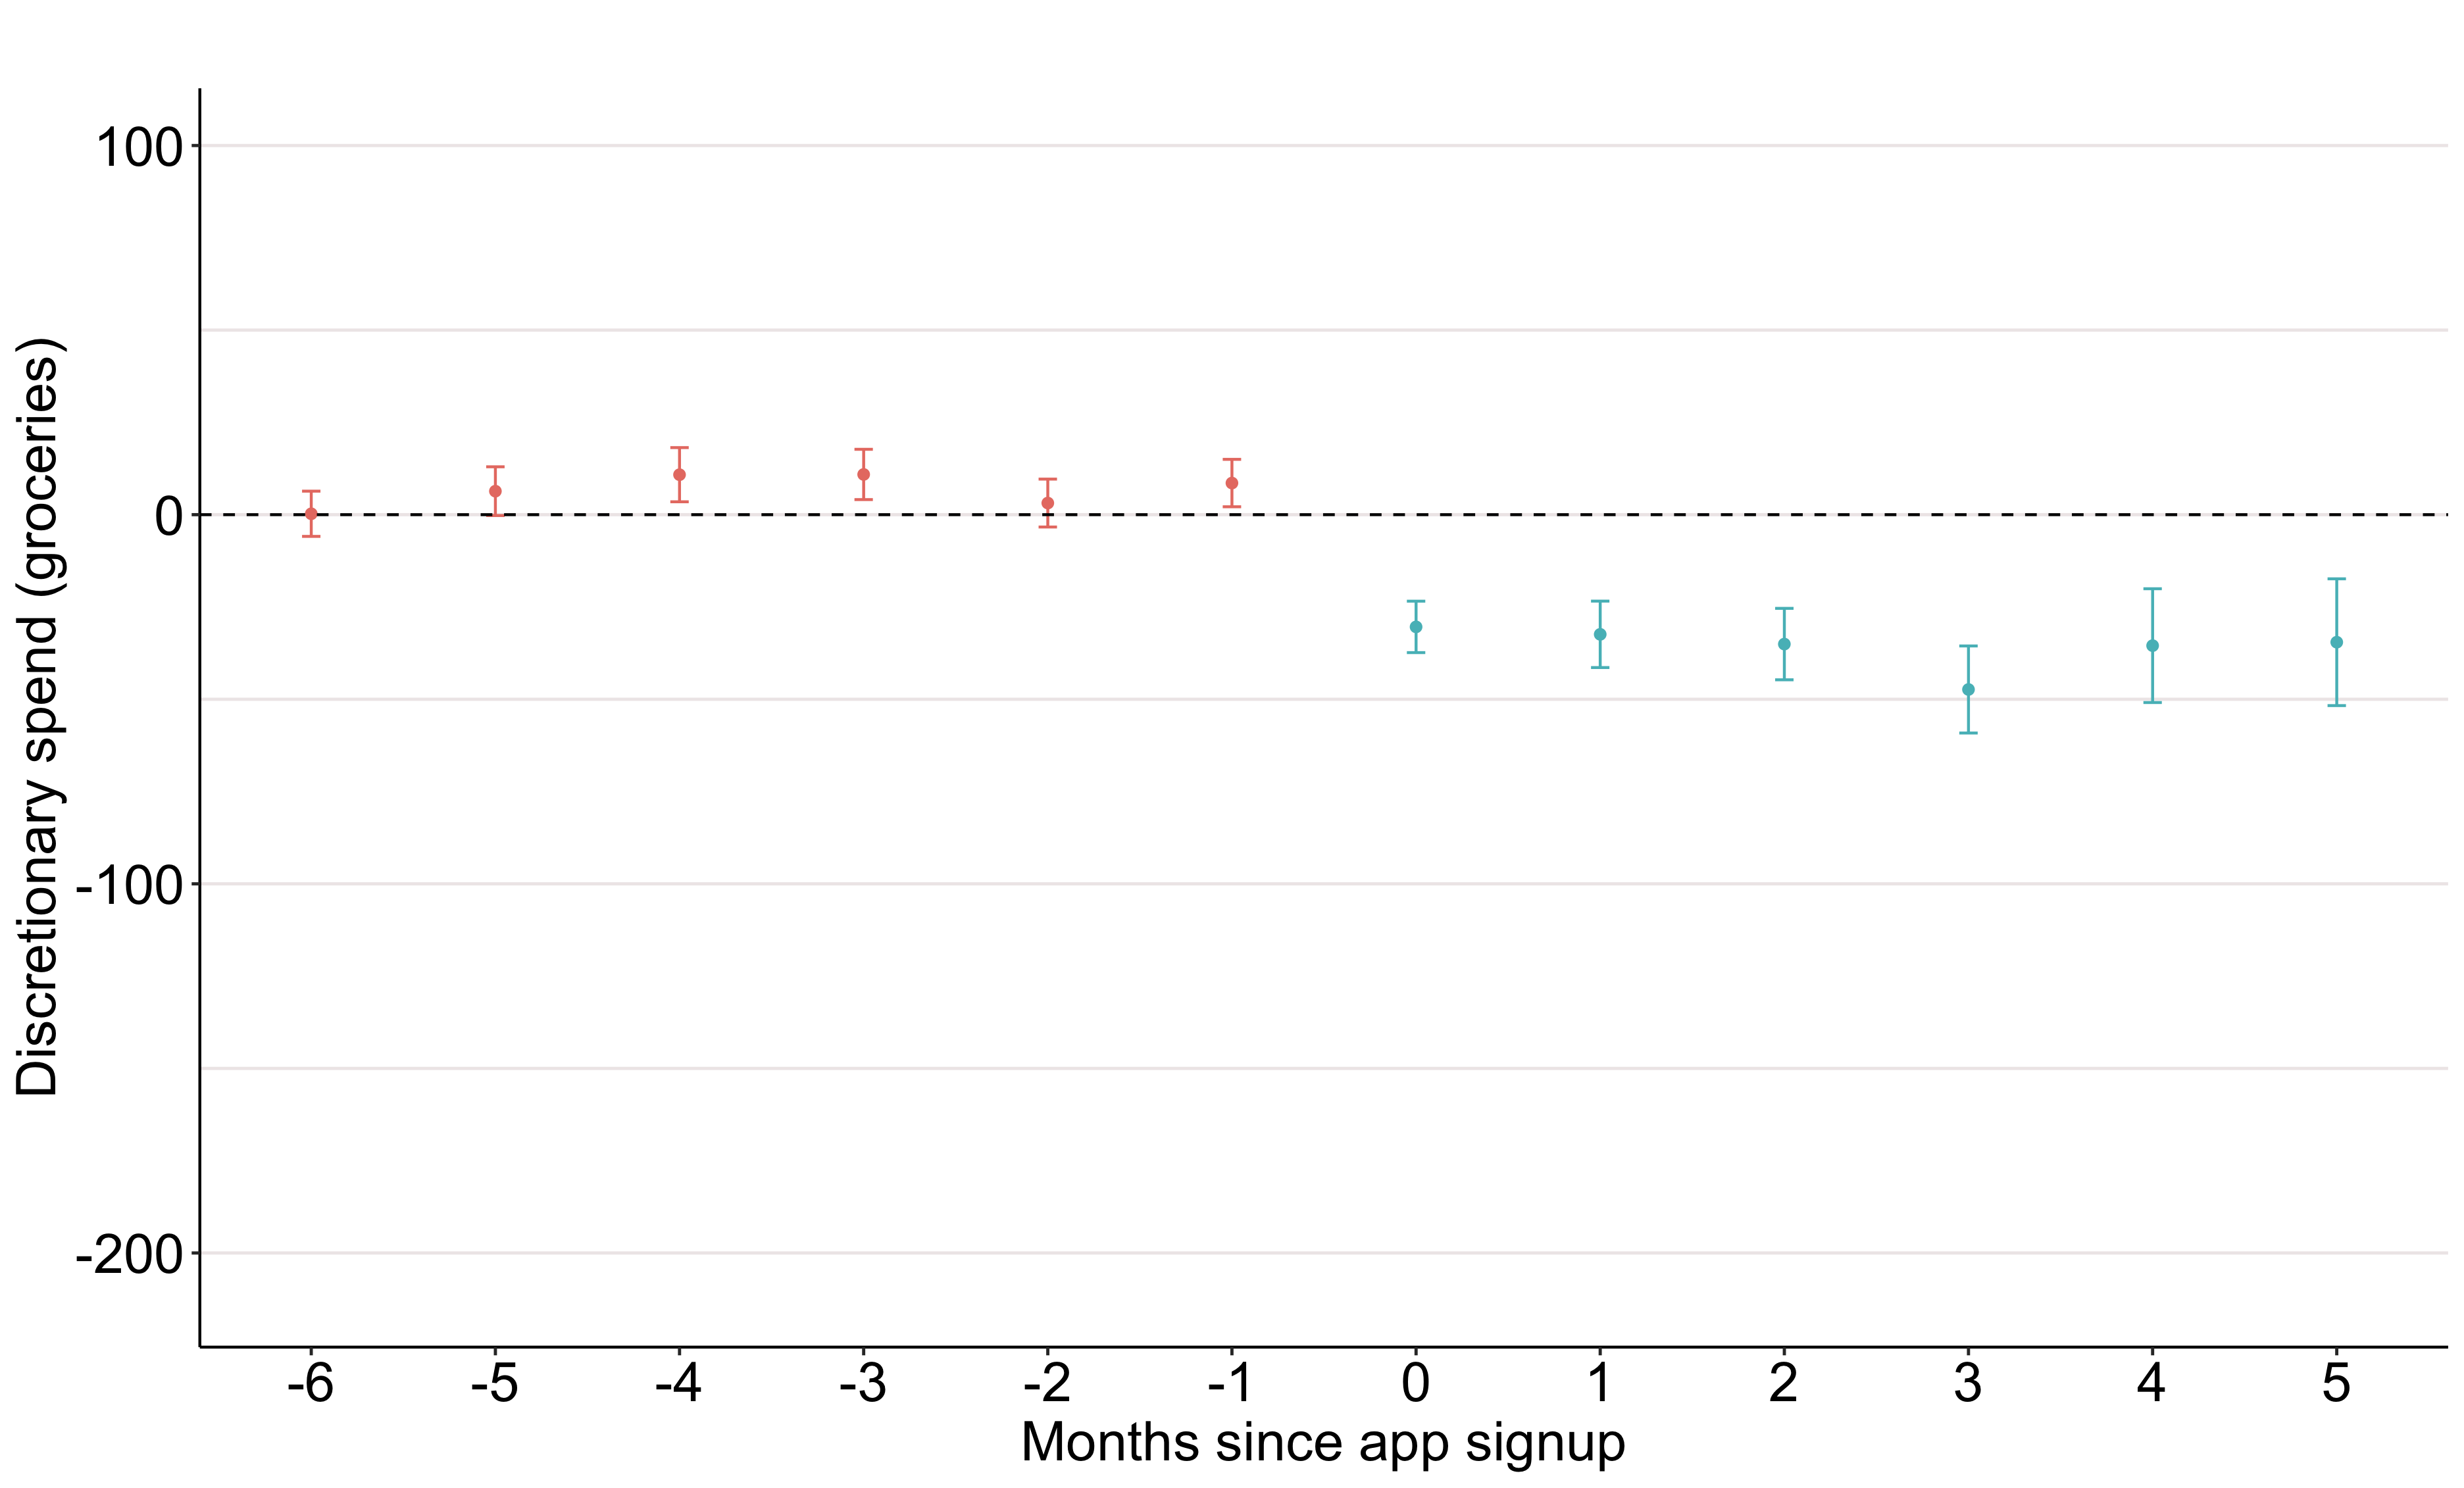
\includegraphics[width=.49\textwidth]{\figdir/disag_dspend_groceries_cond_es.png}
    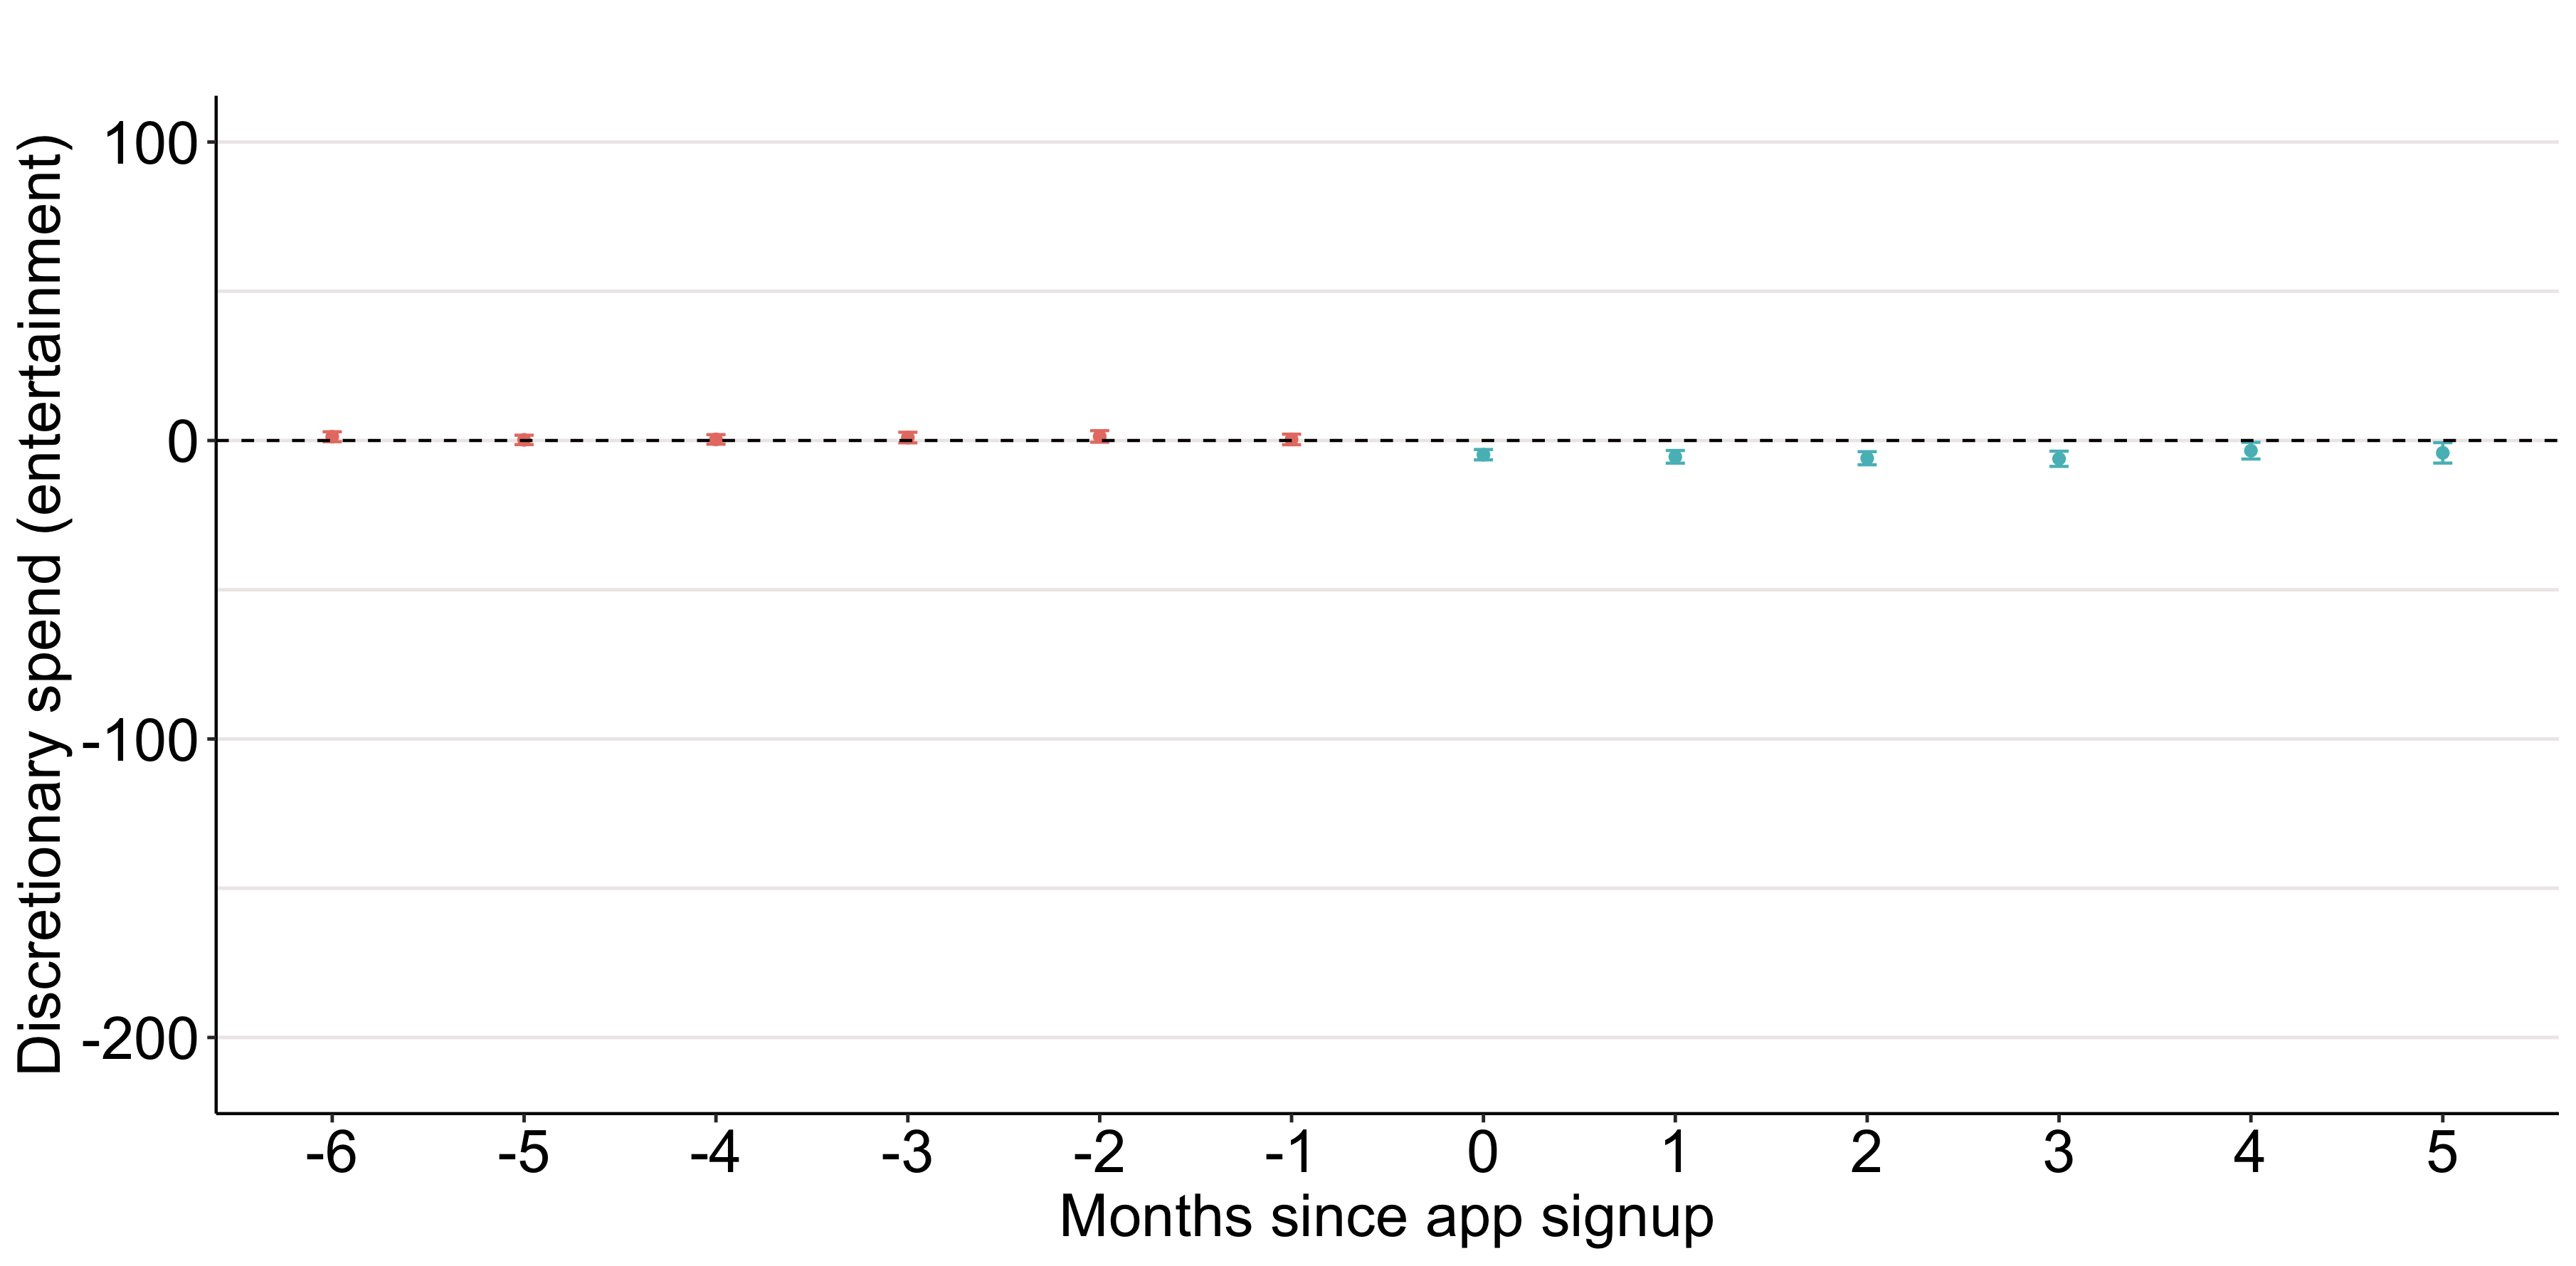
\includegraphics[width=.49\textwidth]{\figdir/disag_dspend_entertainment_cond_es.png}
    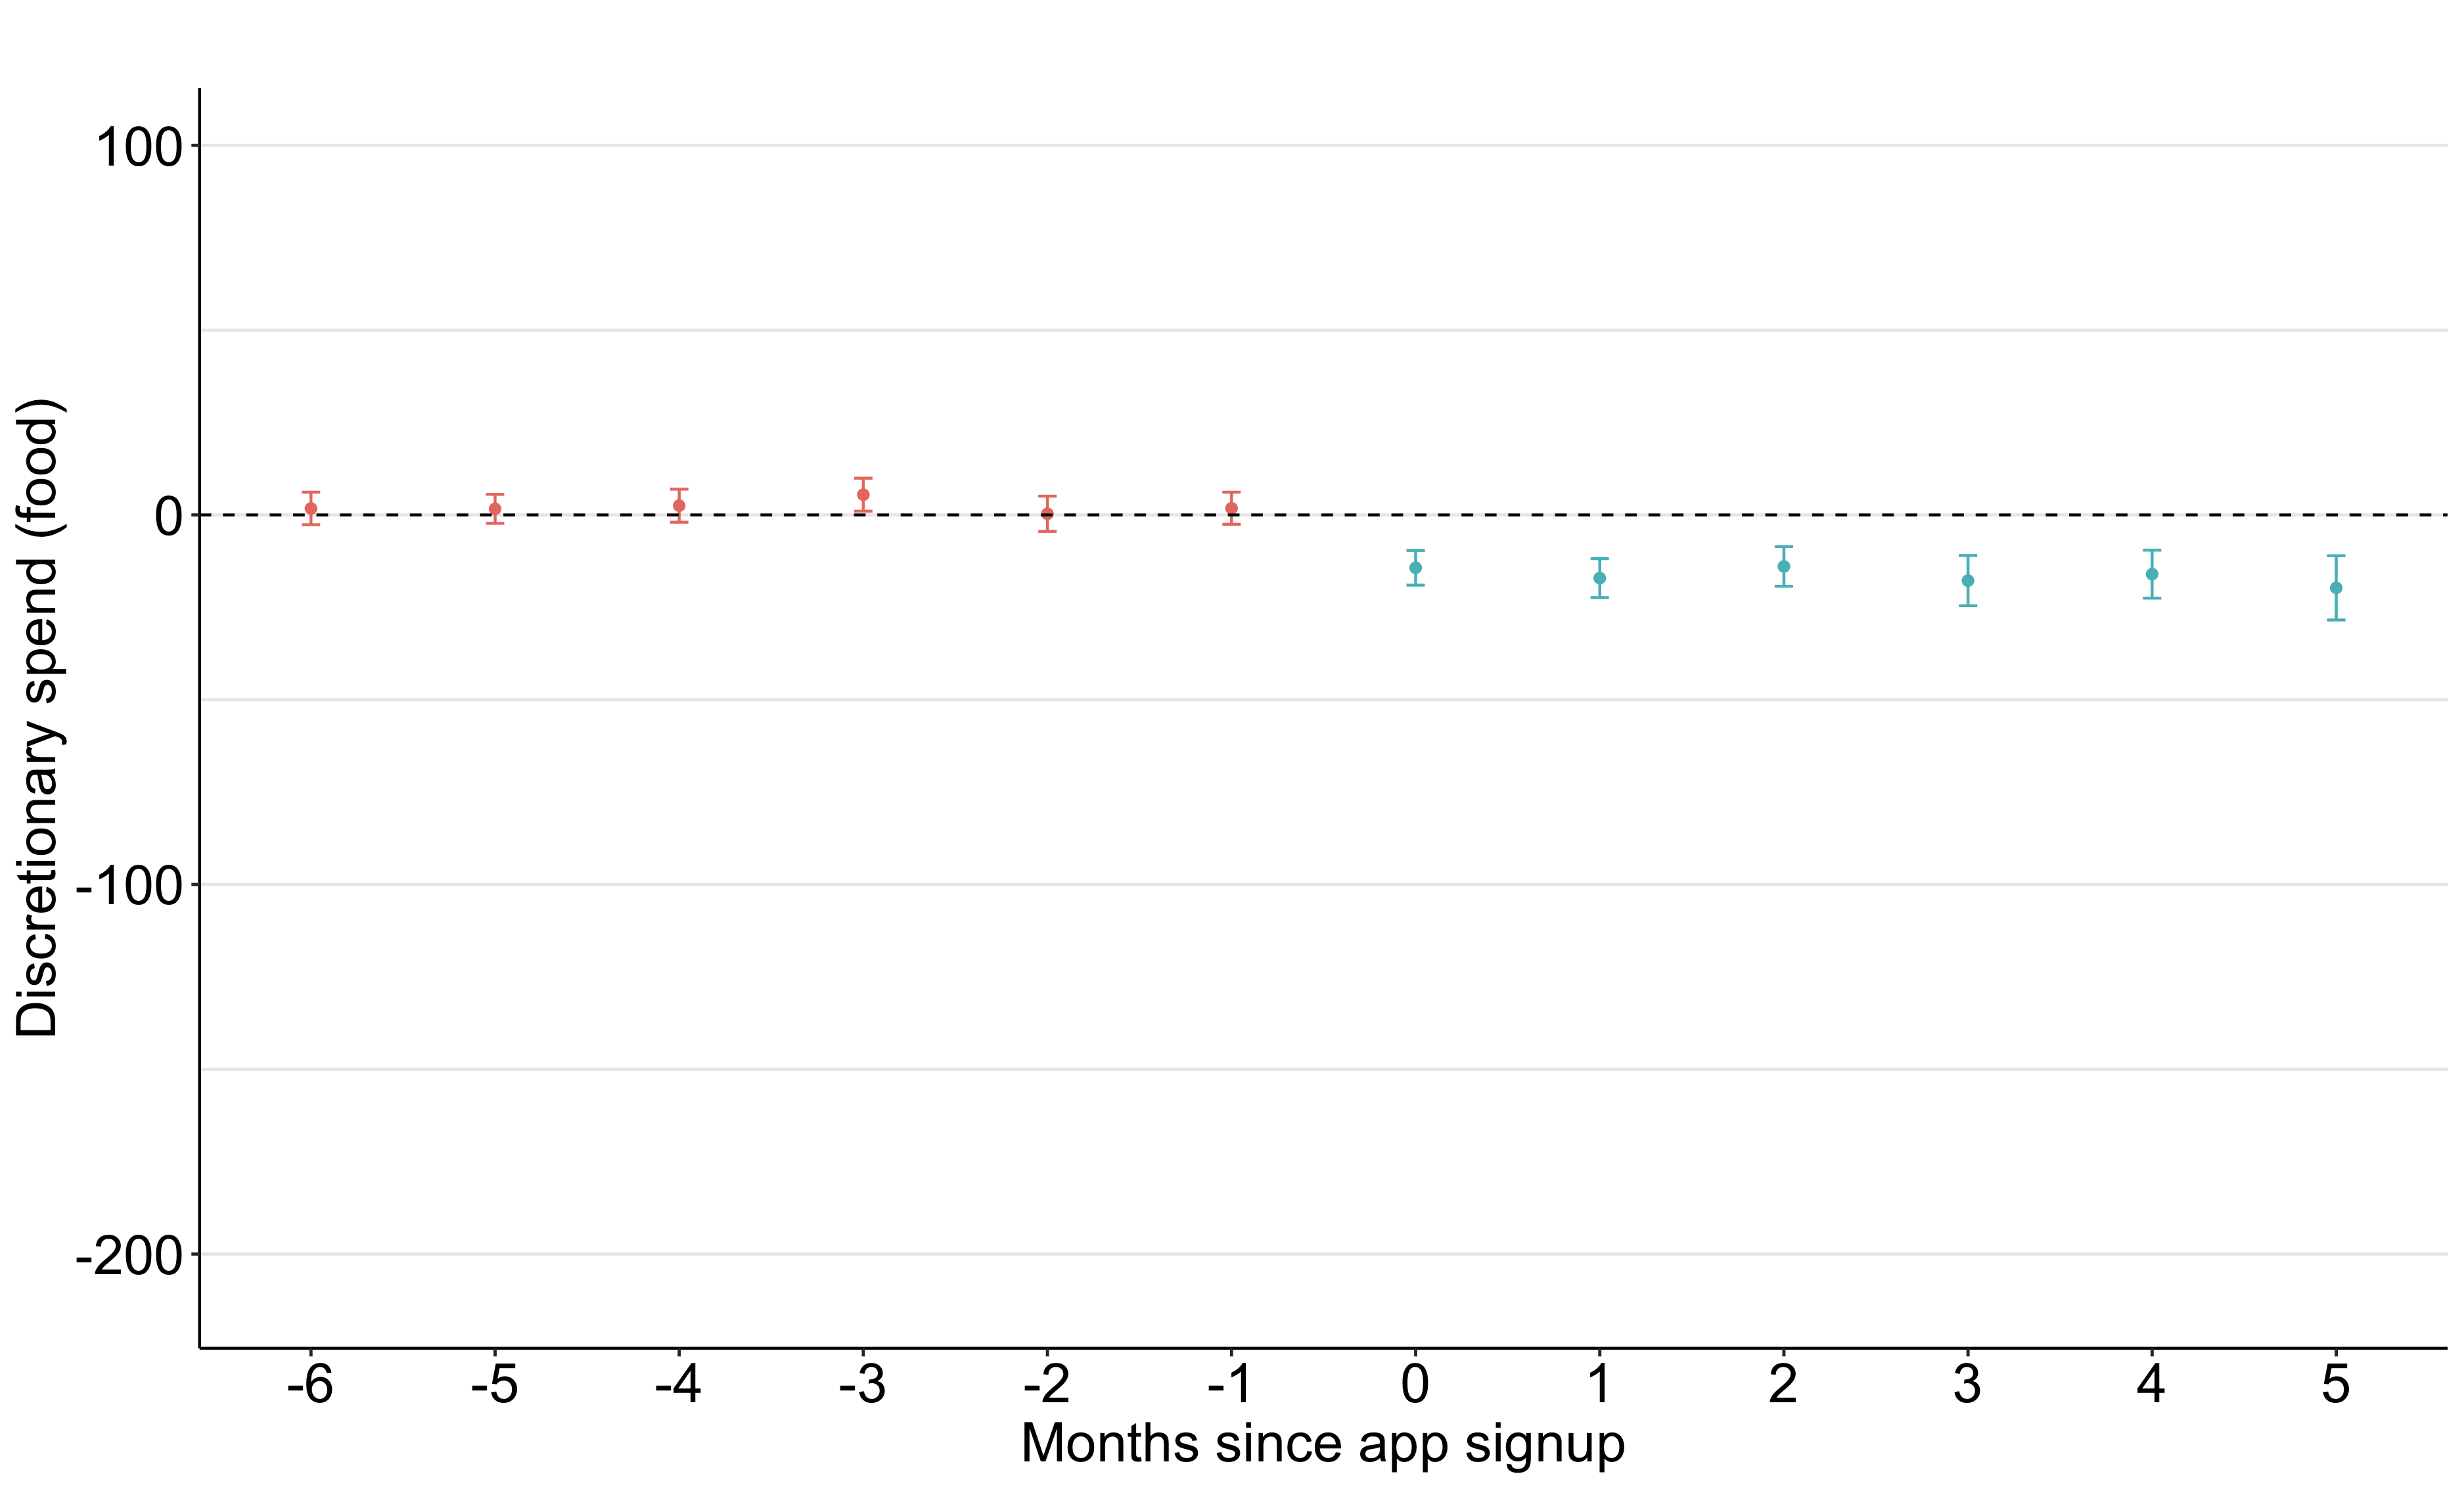
\includegraphics[width=.49\textwidth]{\figdir/disag_dspend_food_cond_es.png}
    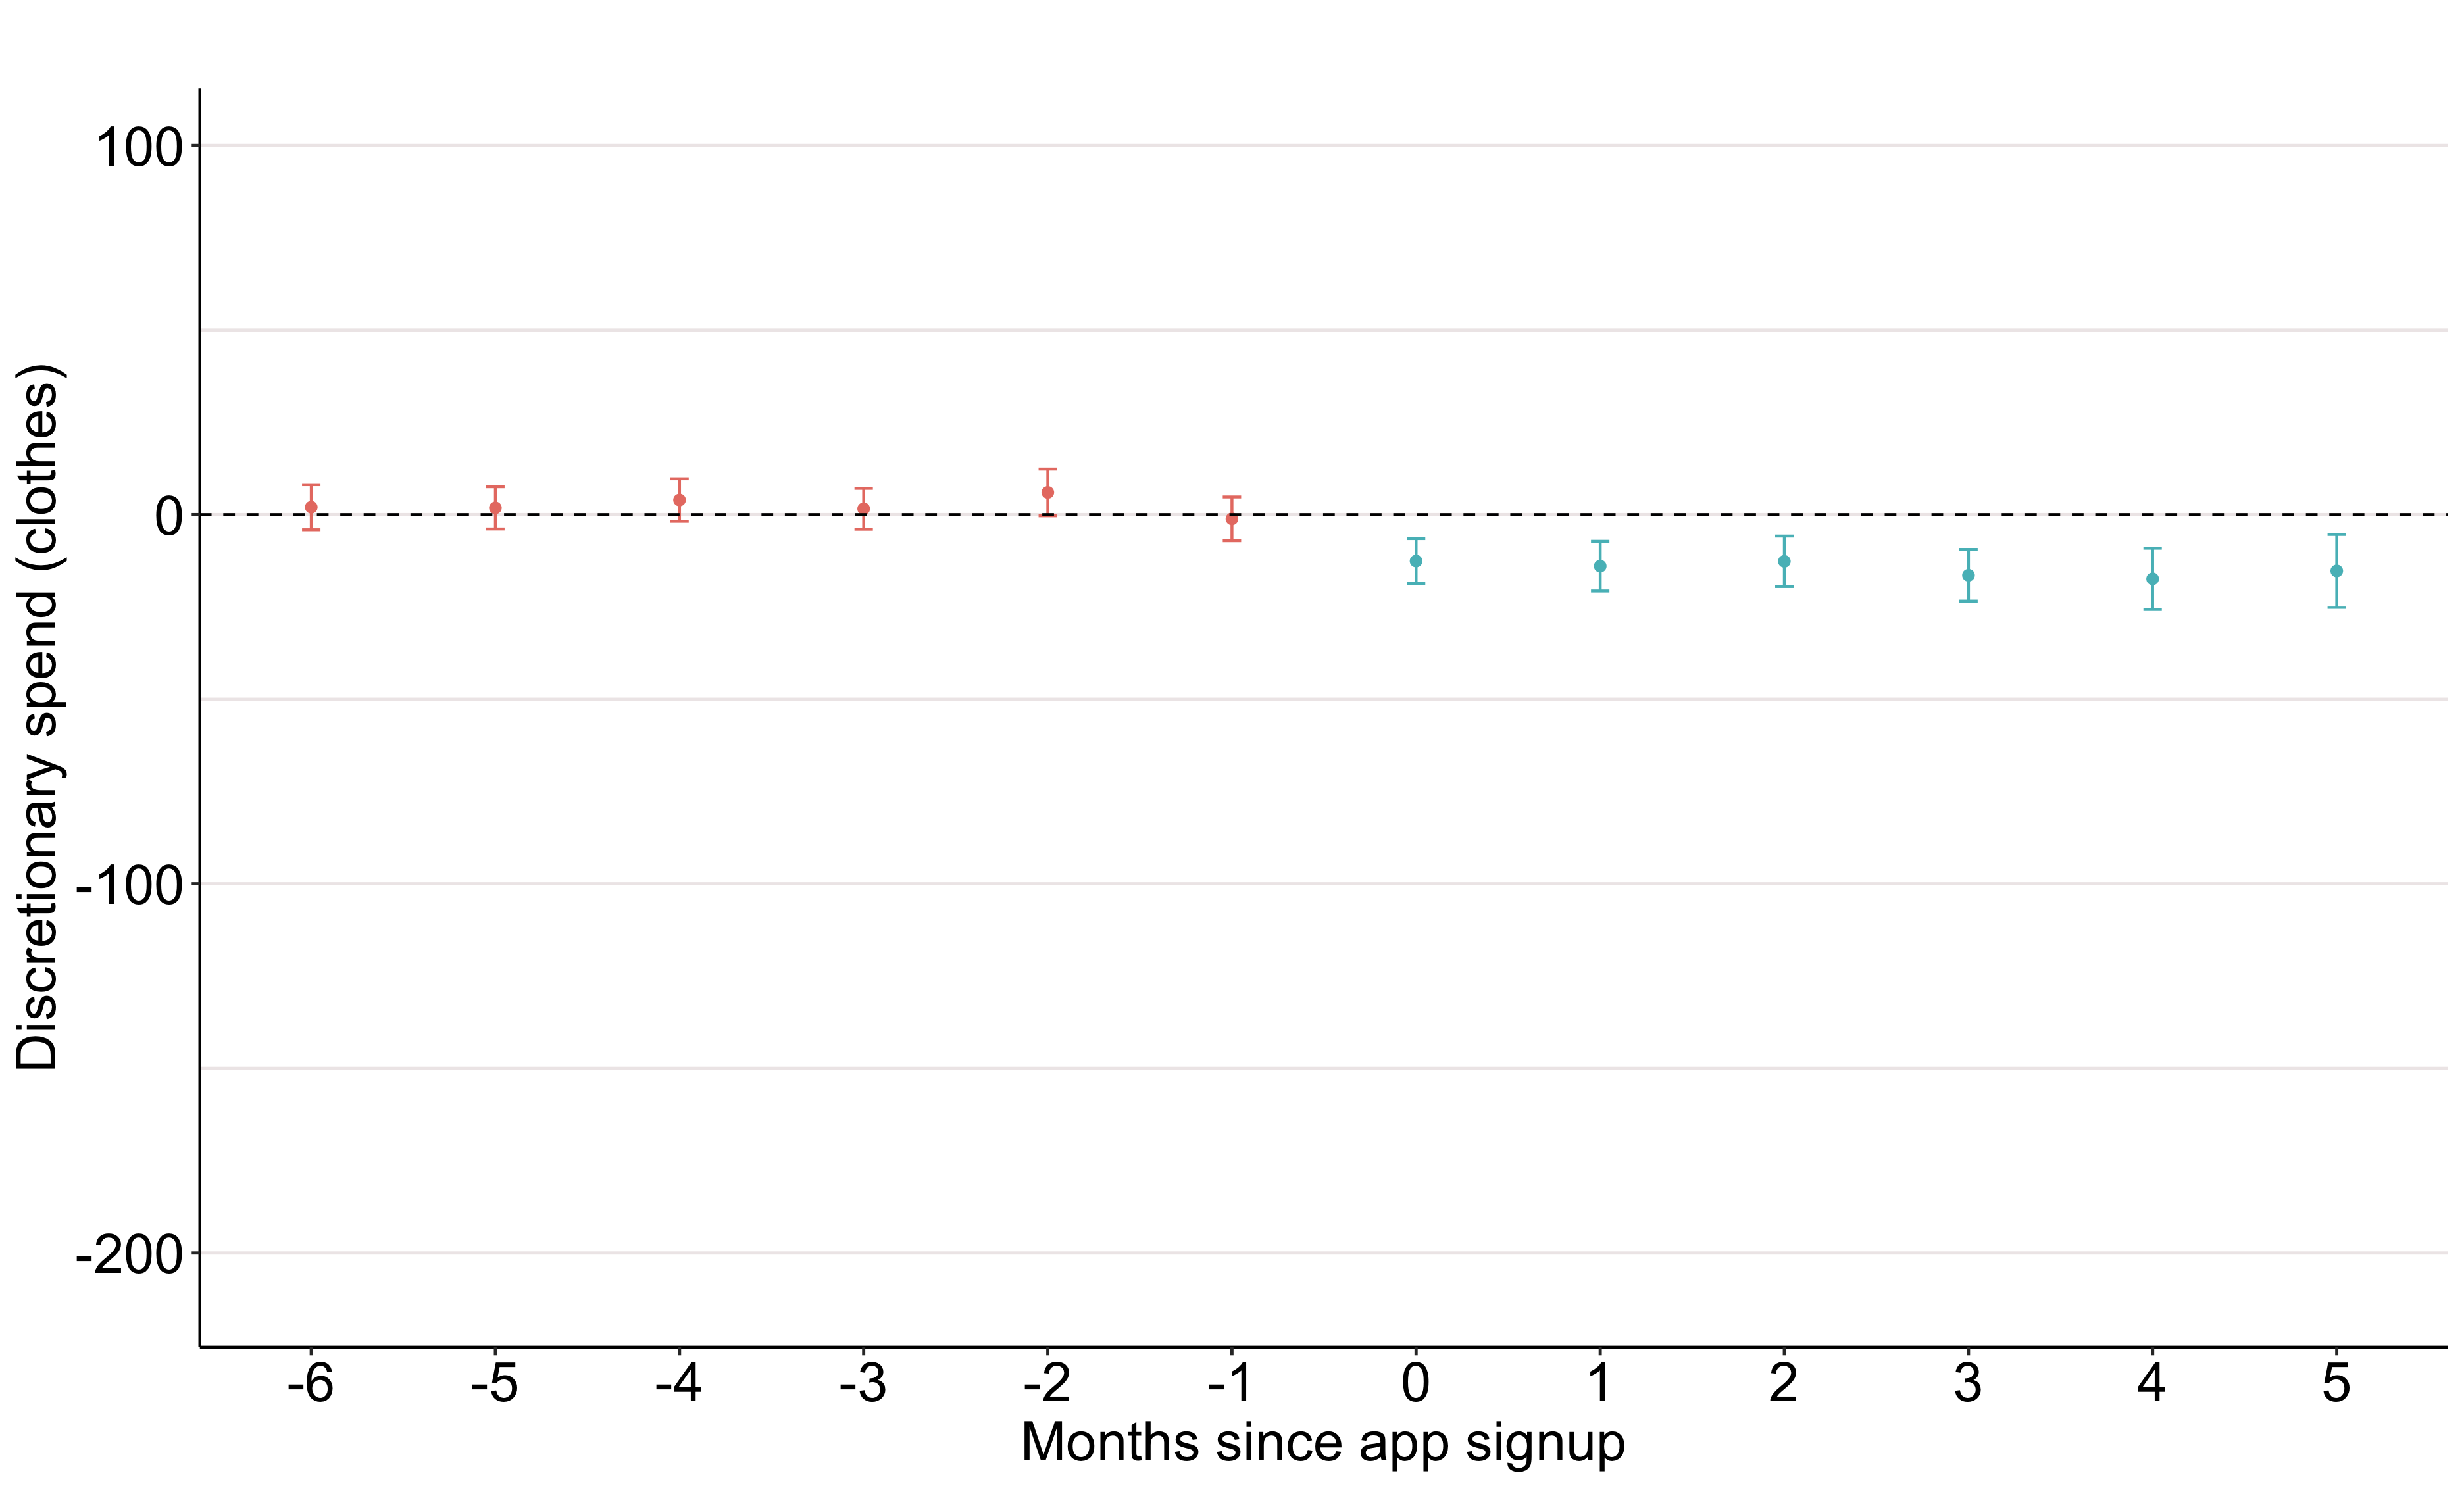
\includegraphics[width=.49\textwidth]{\figdir/disag_dspend_clothes_cond_es.png}
    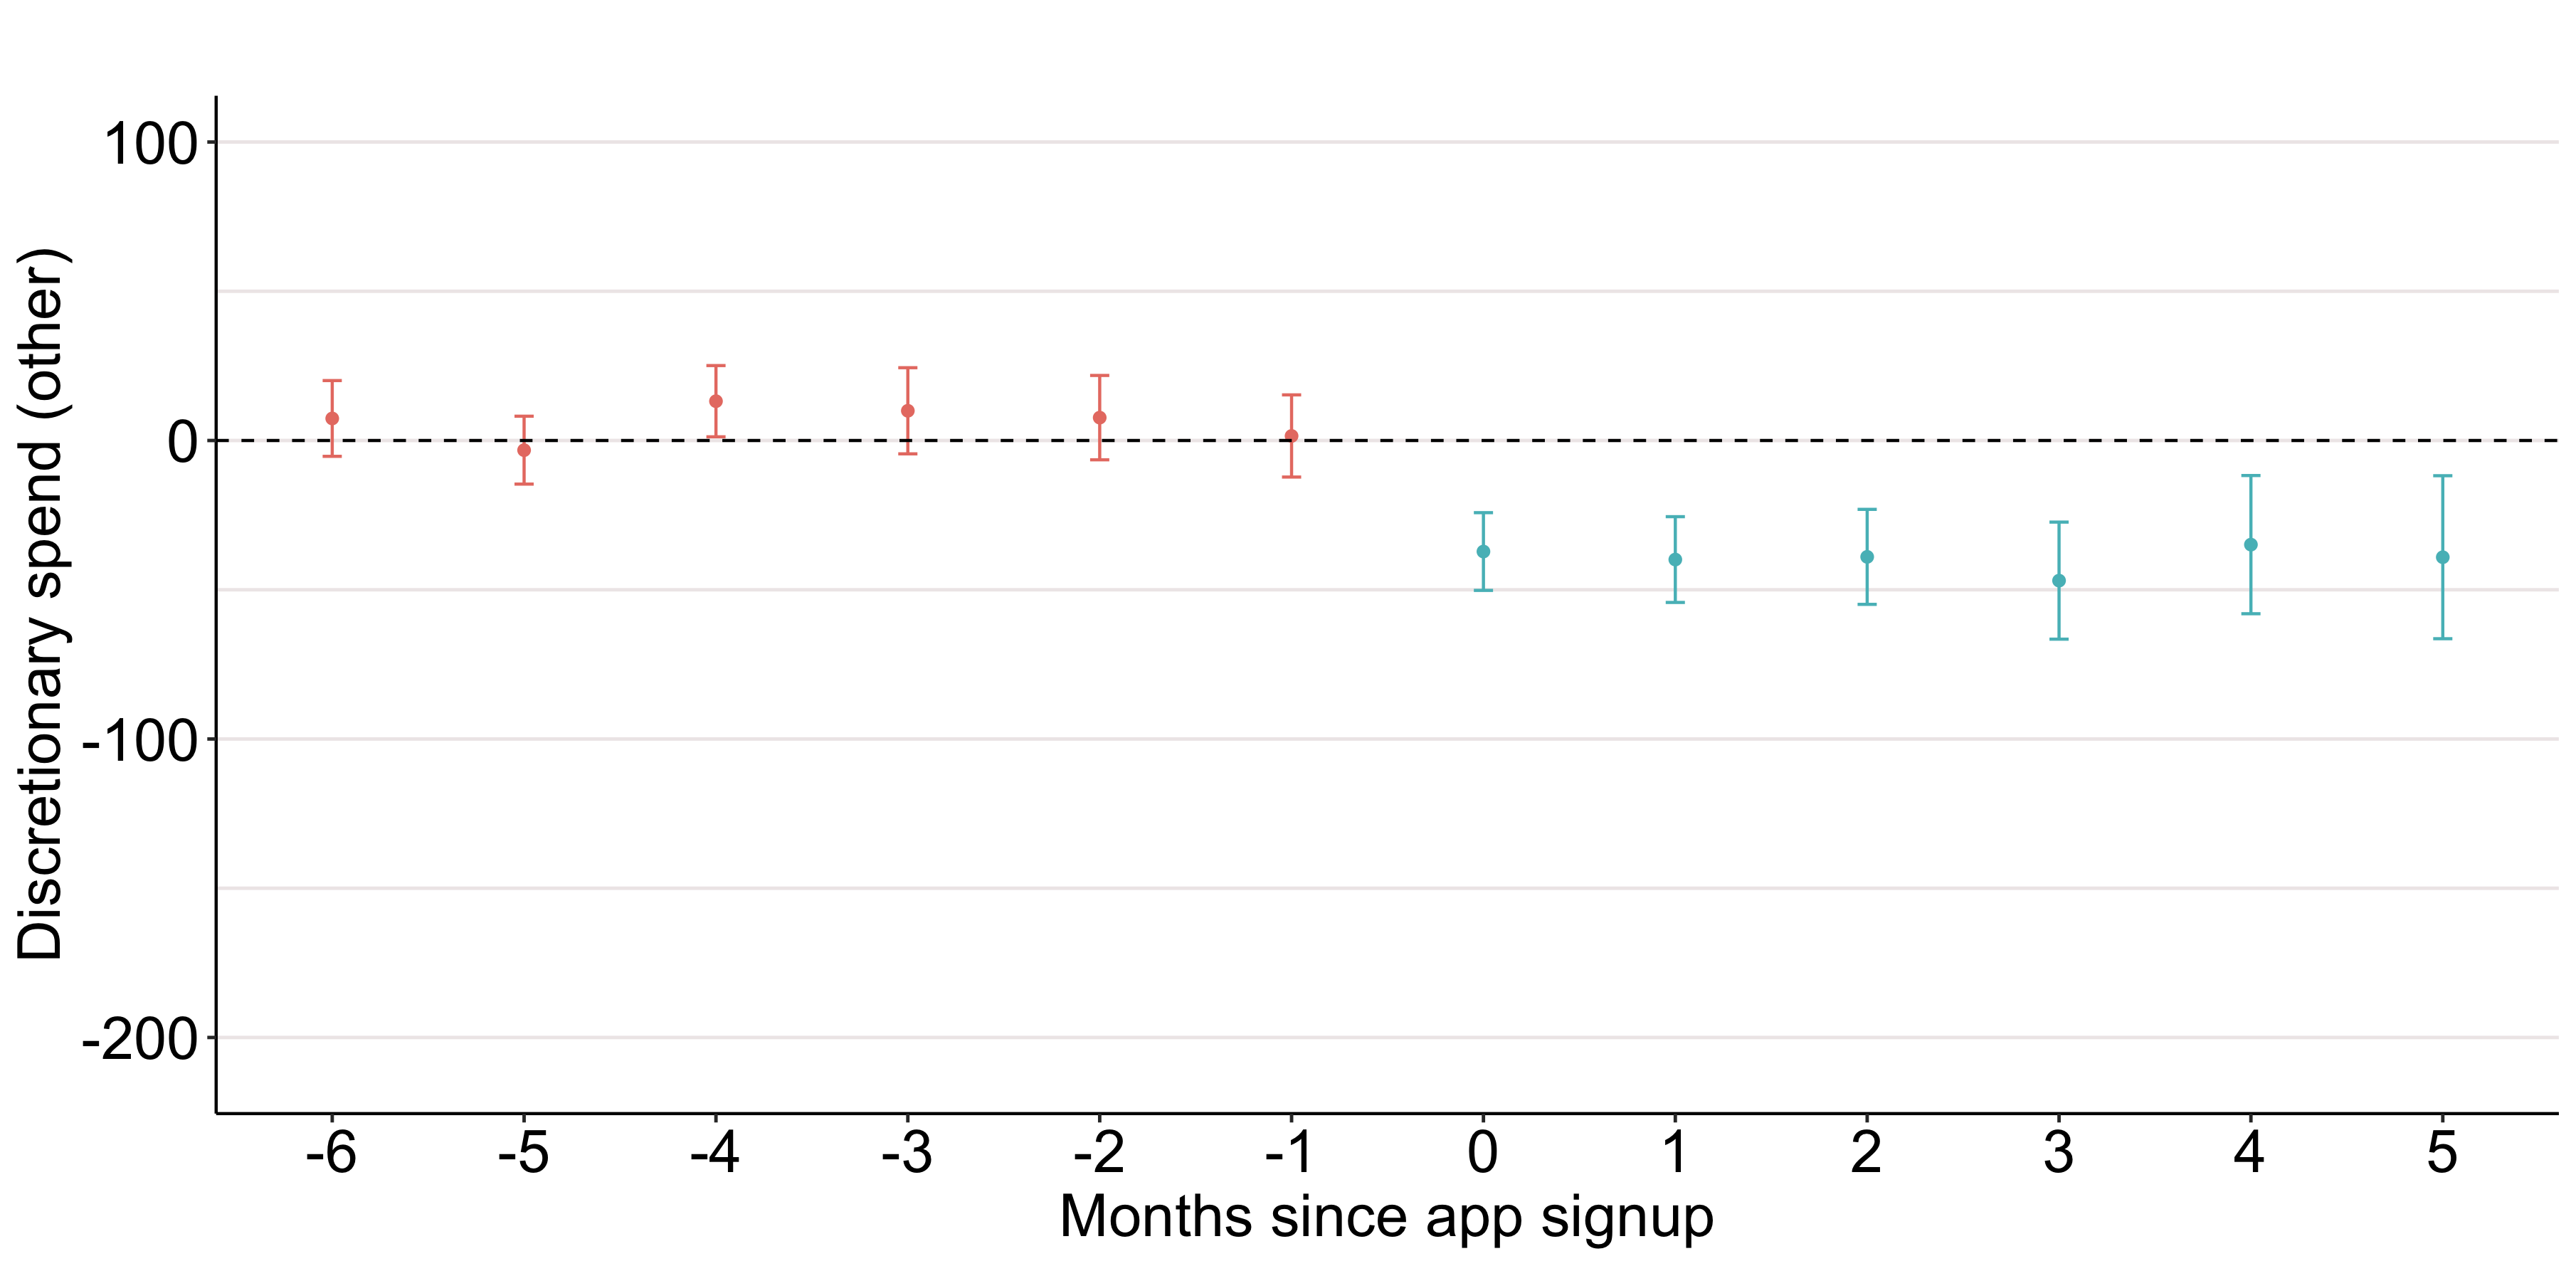
\includegraphics[width=.49\textwidth]{\figdir/disag_dspend_other_cond_es.png}
    \fignote{\textwidth}{Effect of app use on total discretionary spend (for
        reference) and its subgroups. Point estimates represent
        group-time average treatment effects aggregated to periods since
        treatment exposure, as defined in Section~\ref{sec:estimation}. Red
        lines represent point estimates and uniform 95\% confidence bands for
        pre-treatment periods allowing for clustering at the user level. If the
        null hypothesis that parallel trends hold in all periods is correct,
        these should be equal to zero. Blue lines provide similar information
    for post-treatment periods.}
\end{figure}

The second interesting way to disaggregate discretionary spend is into
different component groups based on the type of spend; for this purpose, I
group transactions into ``groceries'', ``clothes'', ``entertainment'',
``food'', which captures spending on restaurant meals and take-away, and
``other''.\footnote{The list used to classify transactions is available on
    \href{https://github.com/fabiangunzinger/mdb_eval/blob/f31bfcd7a330188cdd27968d41957ebf5b454099/src/data/aggregators.py\#L389}{Github}.
    I classify transactions tagged by MDB as ``entertainment'' as ``other
discretionary spend'', since many such transactions are purchases with Amazon,
which we cannot precisely classify.} Figure~\ref{fig:disagg_groups} again
reproduces the plot from the main results in the top-left panel for reference
and then plots results for each of the five subgroups. While we can see that users
mainly reduce spending on groceries and the residual category ``other'',
followed by food and clothes, the overall picture that emerges is that these
differences are quite small, and that the overall reduction in discretionary
spend results from changes along all these margins.

\begin{figure}[h]
    \centering
    \caption{Intensive and extensive margin}%
    \label{fig:int_ext_results}
    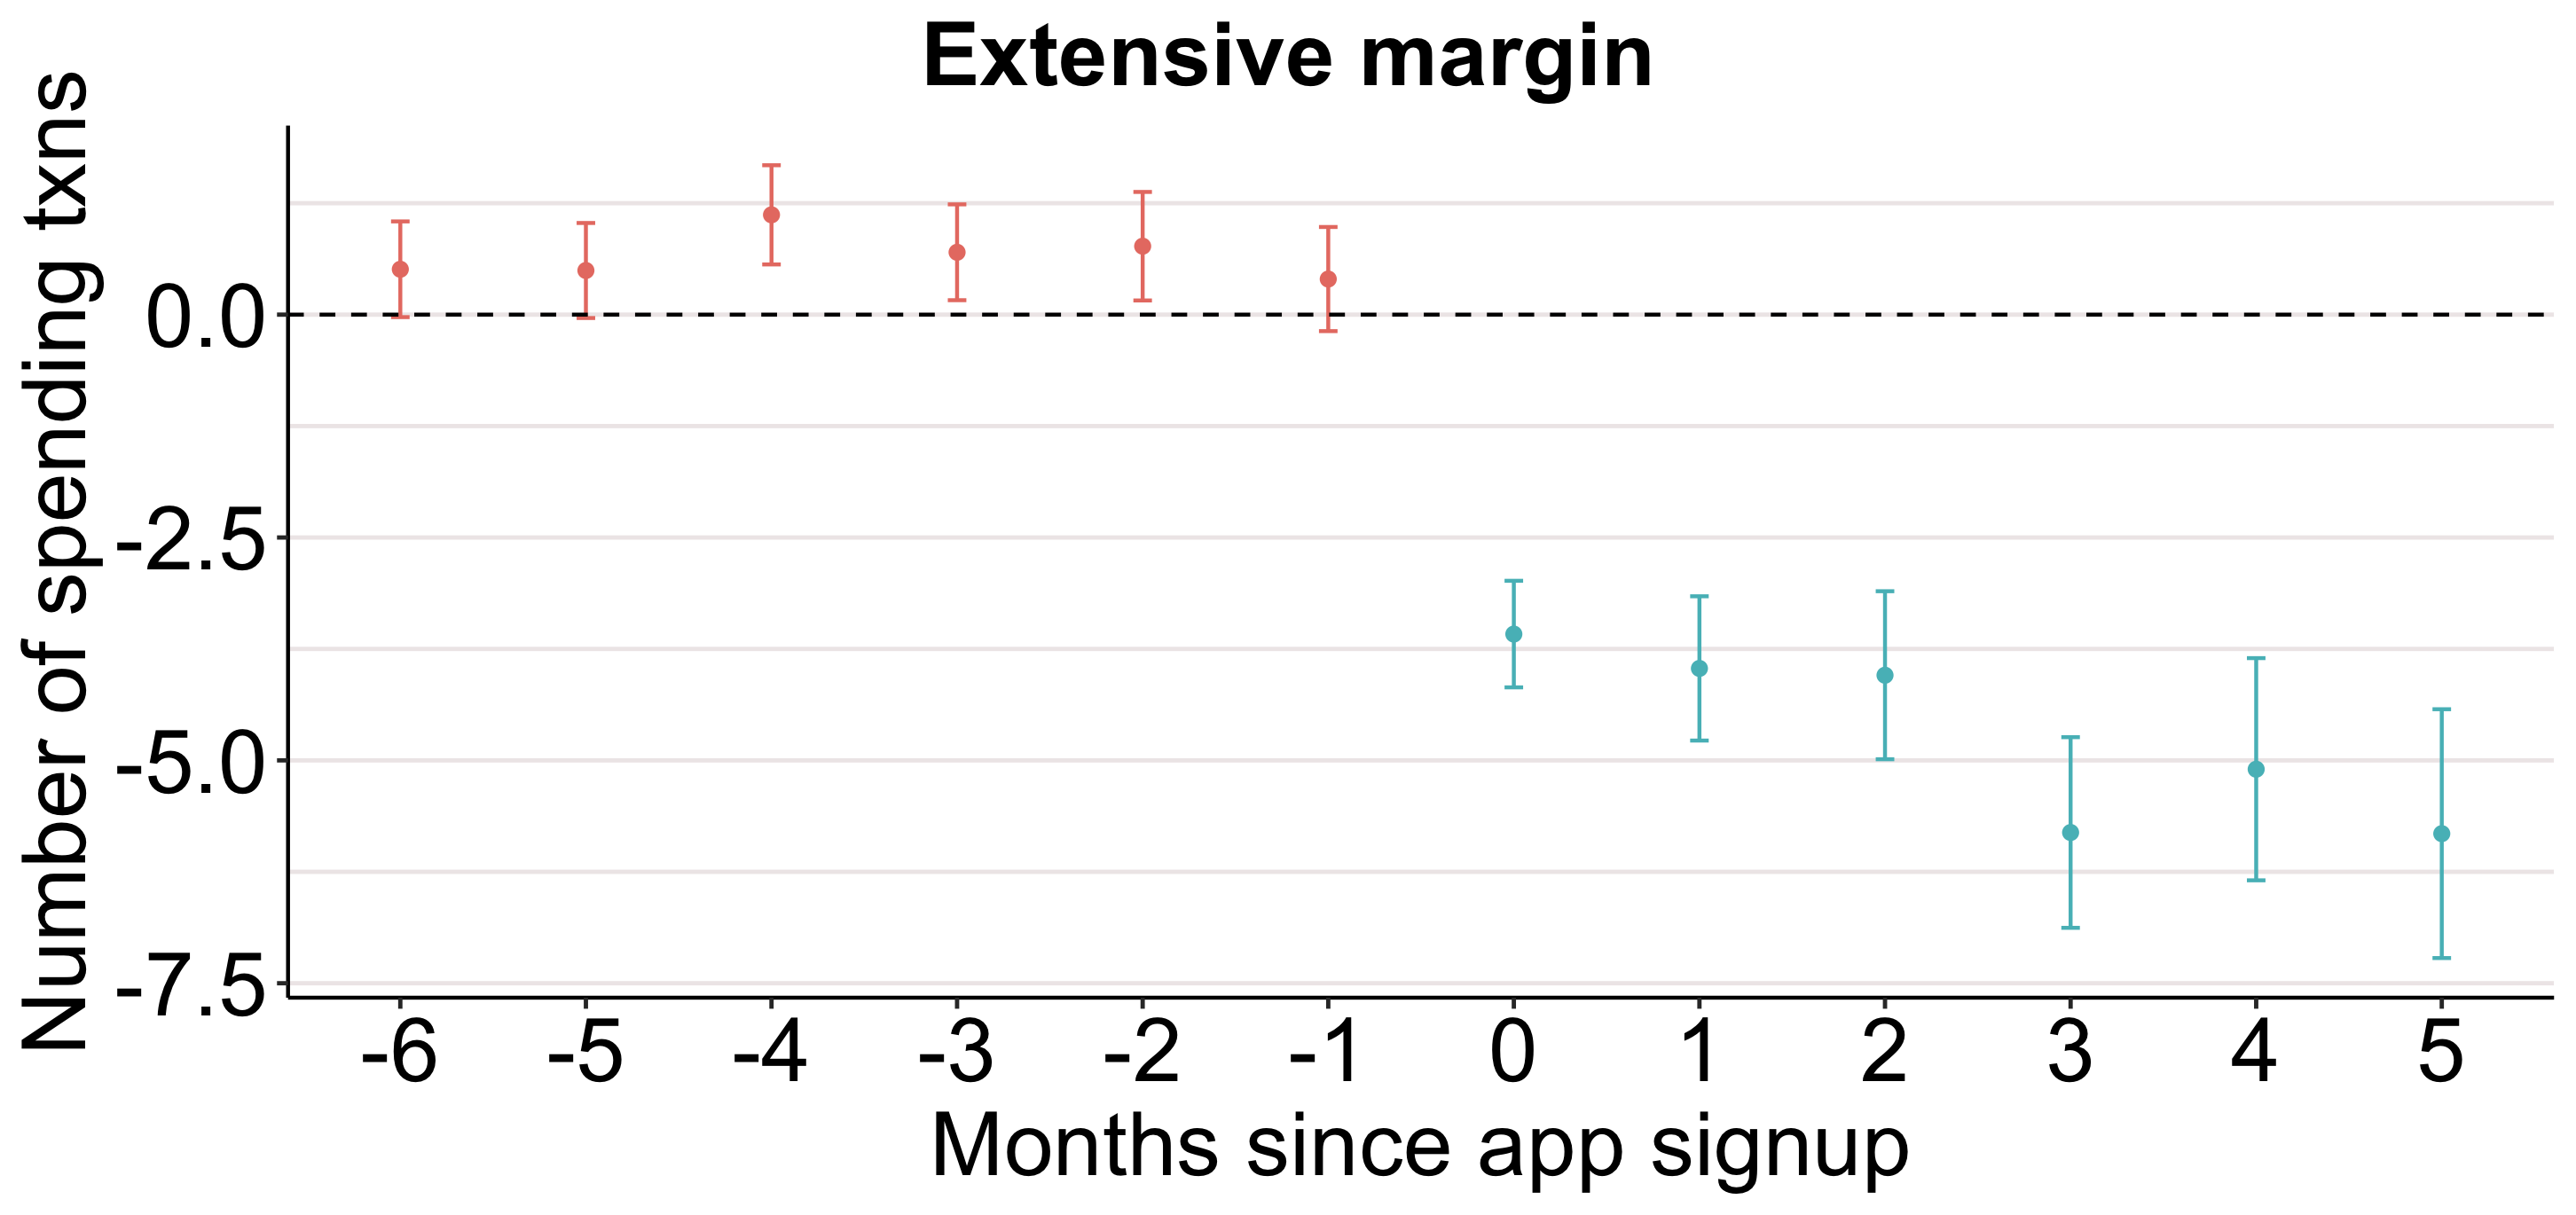
\includegraphics[width=.49\textwidth]{\figdir/dspend_extens_es.png}
    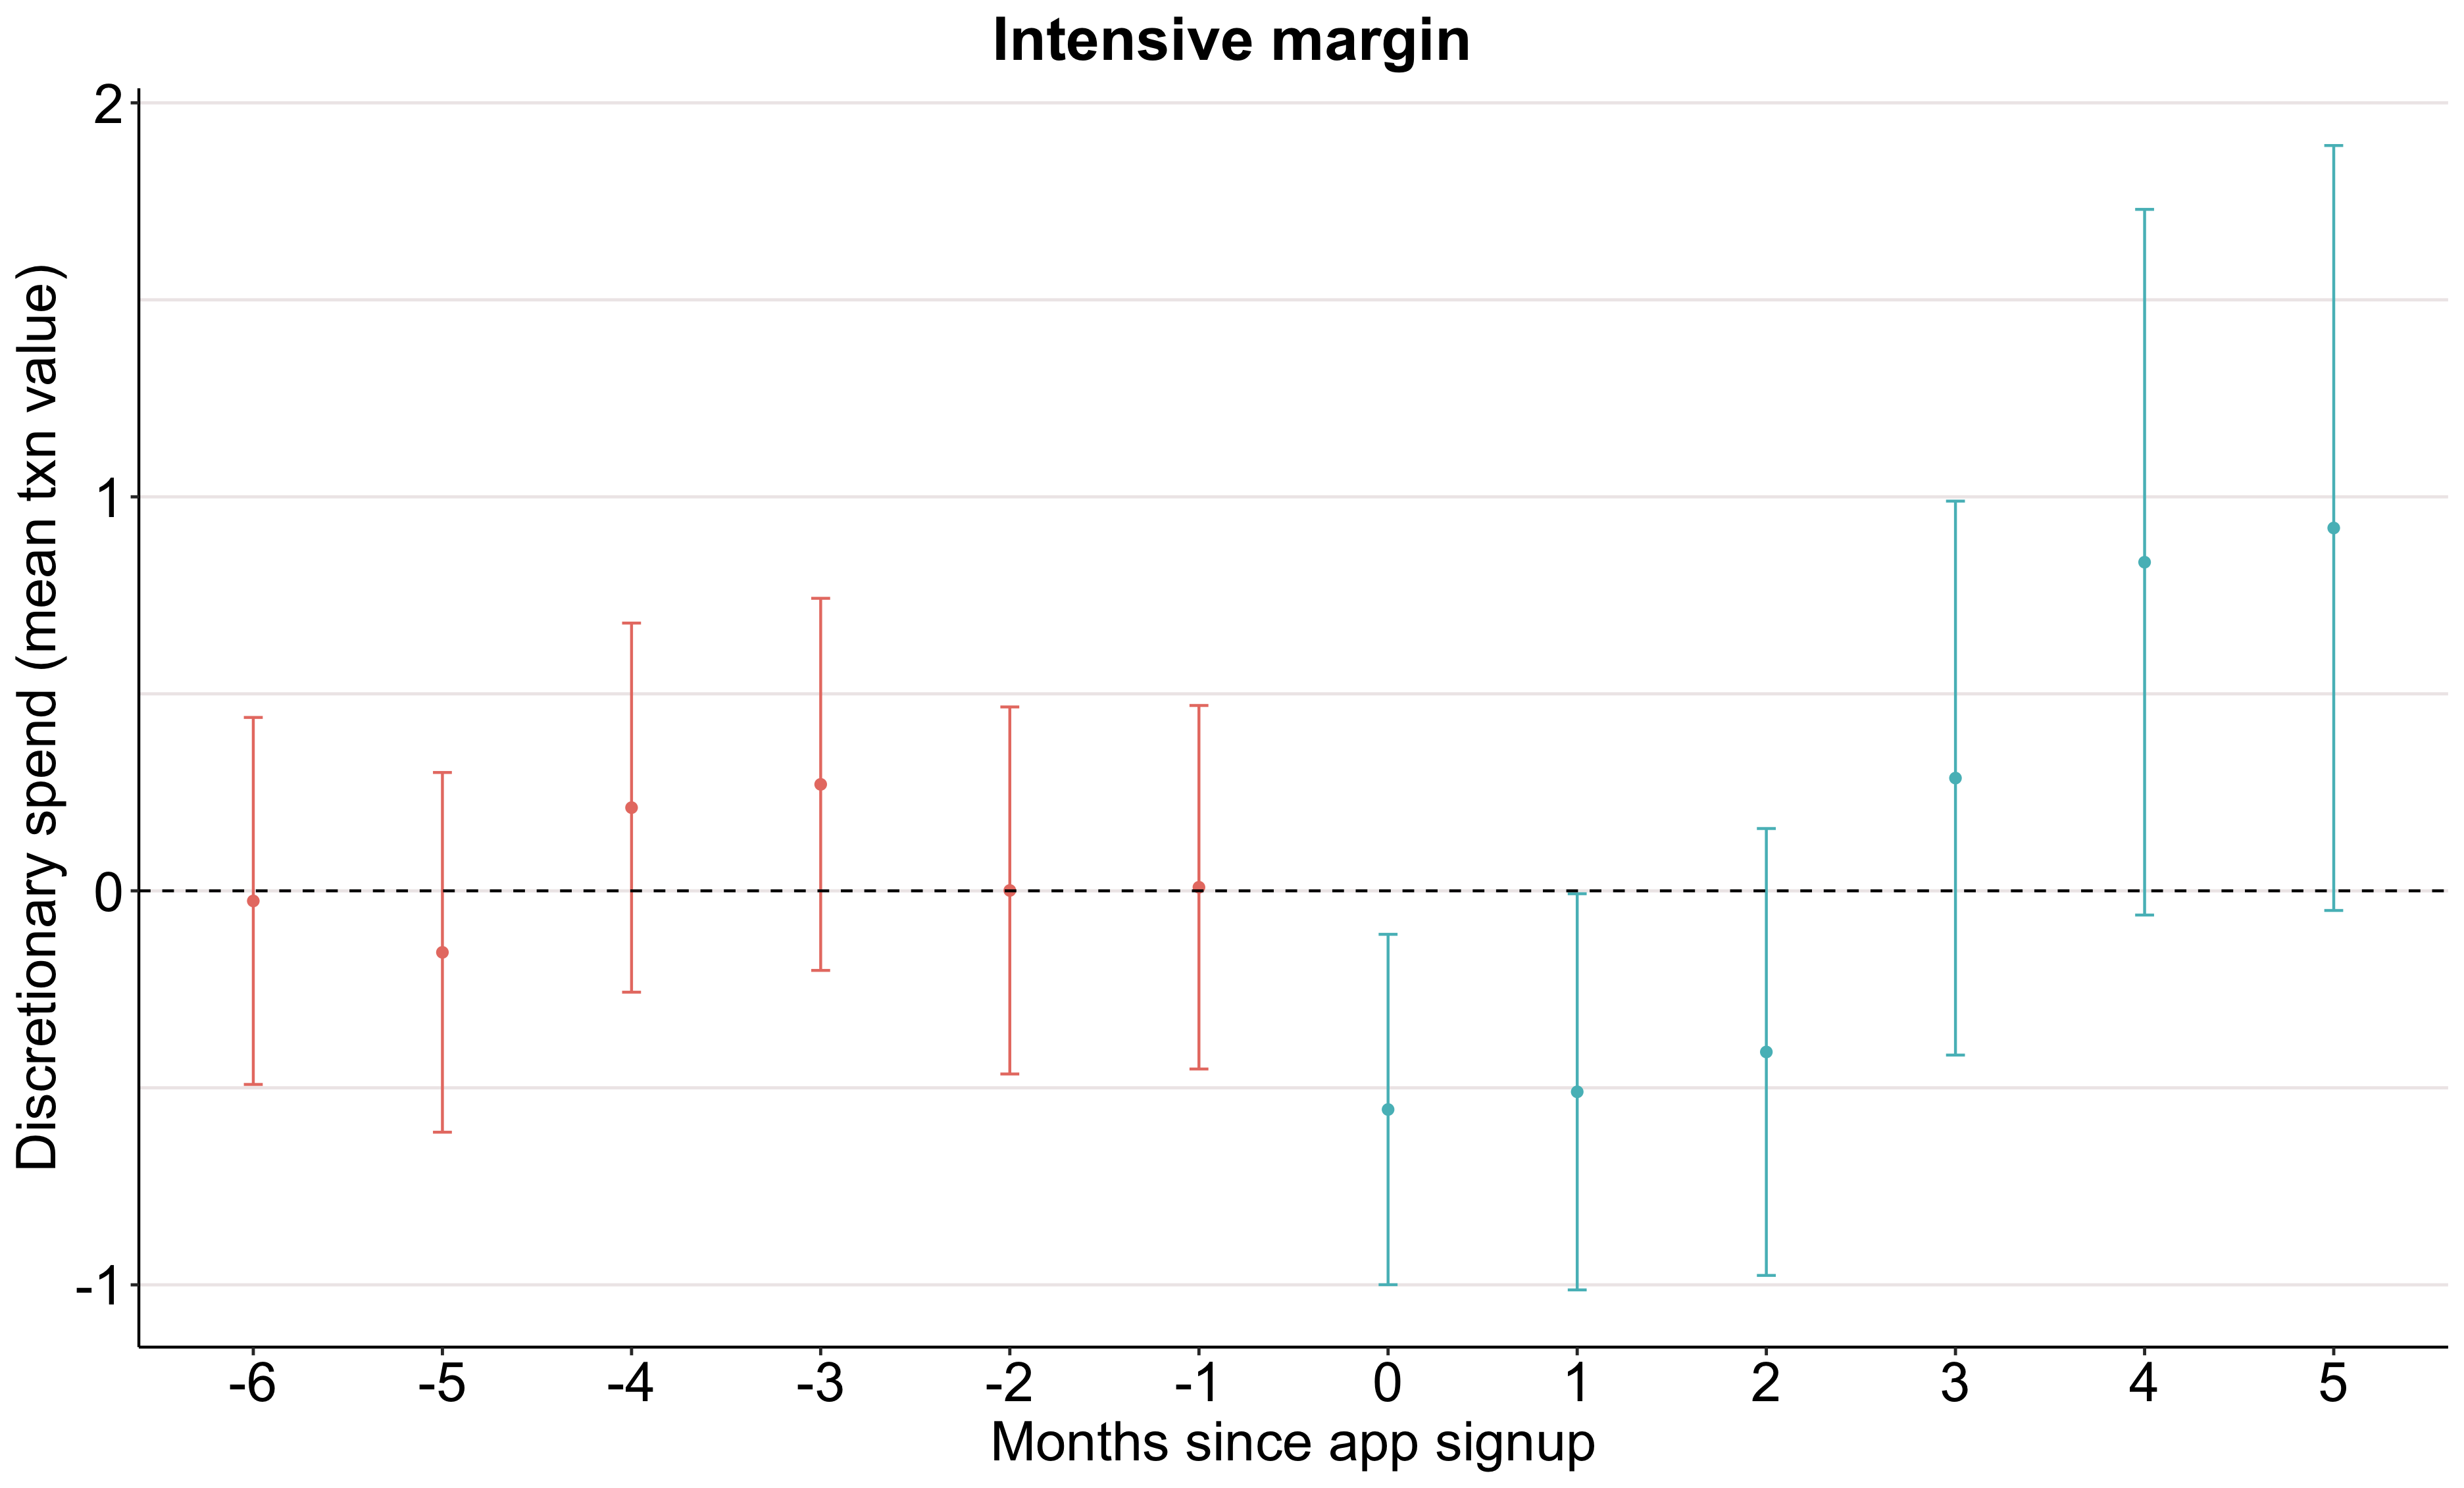
\includegraphics[width=.49\textwidth]{\figdir/dspend_intens_es.png}
    \fignote{\textwidth}{The effect of app use on monthly discretionary spend 
        disaggregated into the effect on the extensive (left column) and
        intensive (right column) margins. The
        extensive margin is the number of discretionary transactions per month,
        and the intensive margin is the average value of a discretionary spend
        transaction. Point estimates represent
        group-time average treatment effects aggregated to periods since
        treatment exposure, as defined in Section~\ref{sec:estimation}. Red
        lines represent point estimates and uniform 95\% confidence bands for
        pre-treatment periods allowing for clustering at the user level. If the
        null hypothesis that parallel trends hold in all periods is correct,
        these should be equal to zero. Blue lines provide similar information
    for post-treatment periods.}
\end{figure}

Finally, it is interesting to consider whether users reduce discretionary spend
along the extensive or the intensive margin -- whether they make fewer
transactions or reduce the average spend per transaction.
Figure~\ref{fig:int_ext_results} shows the number of transactions (the
extensive margin) in the left panel and the average spend per transaction (the
intensive margin) in the right panel. We can see that the reduction in spend is
clearly the result of changes along the extensive margin -- on average, users
make about five fewer discretionary spend purchases per month once they sign up
to MDB. The average transaction value of a discretionary spend purchase in the
data is about \pounds25, adding up to the total effect we find in
Figure~\ref{fig:main_results}.

